\documentclass[a4paper,11pt]{article}

% ========== Encodage & langue ==========
\usepackage[utf8]{inputenc}
\usepackage[T1]{fontenc}
\usepackage[french]{babel}
\usepackage{csquotes}

% ========== Mise en page ==========
\usepackage[margin=2.5cm,headheight=14pt]{geometry}
\usepackage{setspace}
\setstretch{1.15}
\usepackage{fancyhdr}
\usepackage{titlesec}
\usepackage{parskip}

% ========== Typographie ==========
\usepackage{microtype}
\usepackage{lmodern}
\usepackage{xcolor}
\definecolor{nsblue}{HTML}{1F6FB2}
\definecolor{nsgray}{HTML}{4A4A4A}

% ========== Graphiques ==========
\usepackage{graphicx}
\graphicspath{{figures/}{../assets/}}
\usepackage{float}
\usepackage{caption}
\captionsetup{font=small, labelfont=bf, textfont=it, labelsep=colon}
\usepackage{subcaption}

% ========== Tableaux ==========
\usepackage{booktabs}
\usepackage{array}
\usepackage{tabularx}
\usepackage{multirow}

% ========== Maths & unités ==========
\usepackage{amsmath, amssymb, amsfonts}
\usepackage{siunitx}
\sisetup{locale=FR, per-mode=symbol, group-separator={\,}}

% ========== Code source ==========
\usepackage{listings}
\lstdefinestyle{cpp}{
    language=C++,
    basicstyle=\ttfamily\footnotesize,
    keywordstyle=\color{nsblue}\bfseries,
    commentstyle=\color{nsgray}\itshape,
    stringstyle=\color{red!70!black},
    numbers=left,
    numberstyle=\tiny\color{gray},
    numbersep=8pt,
    breaklines=true,
    breakatwhitespace=true,
    frame=single,
    rulecolor=\color{gray!40},
    backgroundcolor=\color{gray!5},
    showstringspaces=false,
    tabsize=4,
    captionpos=b
}
\lstdefinestyle{py}{
    language=Python,
    basicstyle=\ttfamily\footnotesize,
    keywordstyle=\color{nsblue}\bfseries,
    commentstyle=\color{nsgray}\itshape,
    stringstyle=\color{red!70!black},
    numbers=left,
    numberstyle=\tiny\color{gray},
    numbersep=8pt,
    breaklines=true,
    breakatwhitespace=true,
    frame=single,
    rulecolor=\color{gray!40},
    backgroundcolor=\color{gray!5},
    showstringspaces=false,
    tabsize=4,
    captionpos=b
}
\renewcommand{\lstlistingname}{Code}

% ========== Liens ==========
\usepackage[hidelinks]{hyperref}
\hypersetup{
    colorlinks=true,
    linkcolor=nsblue,
    urlcolor=nsblue,
    citecolor=nsblue,
    pdftitle={NeuralSpeech --- Reconnaissance vocale embarquée sur Arduino Due},
    pdfauthor={Équipe NeuralSpeech}
}

% ========== En-têtes ==========
\pagestyle{fancy}
\fancyhf{}
\fancyhead[L]{\textit{NeuralSpeech}}
\fancyhead[R]{ING3 S6 --- Calcul Embarqué}
\fancyfoot[C]{\thepage}
\renewcommand{\headrulewidth}{0.3pt}

% ========== Macros projet ==========
\newcommand{\etref}[1]{\textbf{ET#1}}
\newcommand{\fpref}[1]{\textbf{FP#1}}
\newcommand{\TODO}[1]{\textbf{\textcolor{red}{[TODO : #1]}}}
\newcommand{\FILLED}[1]{\textcolor{green!50!black}{\checkmark\ #1}}

% ========== Métadonnées ==========
\title{\vspace{-2cm}
       \Huge\textbf{\textcolor{nsblue}{NeuralSpeech}}\\[0.3em]
       \Large Reconnaissance vocale embarquée sur Arduino Due\\[0.8em]
       \normalsize Projet d'Électronique --- ING3 S6 Calcul Embarqué}
\author{Équipe NeuralSpeech \\
        \small Gaspard Boucharlat \\
        \small \TODO{compléter avec les 3 autres membres}\\[1em]
        \textit{École Centrale d'Électronique --- ECE Paris}}
\date{2026}

\begin{document}

\maketitle
\thispagestyle{empty}

\vfill
\begin{center}
    \small
    \textit{Ce rapport documente la conception et la réalisation d'un système de reconnaissance vocale embarqué sur microcontrôleur Arduino Due (SAM3X8E), dans le cadre du projet d'électronique du semestre 6.}
\end{center}
\vfill

\newpage
\tableofcontents
\newpage

% ========== Contenu ==========
\section*{Résumé}
\addcontentsline{toc}{section}{Résumé}

\TODO{Rédiger en fin de projet — 200 à 300 mots résumant : contexte, objectif, chaîne technique (ADC, filtrage, MFCC, CNN), résultats (taux de reconnaissance, temps de traitement), conclusions principales.}

\vspace{1em}

\textbf{Mots-clés :} reconnaissance vocale, systèmes embarqués, Arduino Due, SAM3X8E, MFCC, réseau de neurones convolutionnel, traitement du signal temps réel.

\newpage

\section{Introduction}

\subsection{Contexte et problématique}

Dans le cadre du module de Calcul Embarqué du semestre 6 (ING3) à l'ECE Paris, il est demandé de concevoir un système de reconnaissance vocale fondé sur une intelligence artificielle s'exécutant \emph{intégralement} sur une carte Arduino Due (SAM3X8E, \SI{84}{\mega\hertz}, \SI{96}{\kibi\byte} de SRAM). Le projet, nommé \textbf{NeuralSpeech}, s'inscrit dans la continuité pédagogique des modules de traitement numérique du signal, d'architecture microcontrôleur et d'apprentissage automatique.

La ligne rouge à ne pas franchir est formelle : \emph{la reconnaissance doit se faire sur l'Arduino Due impérativement}. Un projet fonctionnel sur PC mais incapable de tourner sur le microcontrôleur entraîne un malus forfaitaire de -12 points sur la note finale.

\subsection{Objectifs du projet}

L'objectif est de réaliser une chaîne complète de traitement audio, depuis la captation analogique jusqu'à la classification temps réel :
\begin{enumerate}
    \item Numériser un signal audio à \SI{32}{\kilo\hertz} via l'ADC intégré.
    \item Filtrer numériquement puis sous-échantillonner à \SI{8}{\kilo\hertz}.
    \item Valider l'enregistrement par export sur Audacity.
    \item Extraire les coefficients MFCC caractéristiques du timbre vocal.
    \item Entraîner un réseau de neurones convolutionnel en Python.
    \item Embarquer l'inférence sur l'Arduino Due et signaler le mot détecté par des LEDs.
\end{enumerate}

\subsection{Cadre et contraintes (ET1 à ET9)}

Le sujet impose neuf exigences techniques (ET) non négociables, récapitulées au tableau~\ref{tab:et}.

\begin{table}[H]
\centering
\small
\begin{tabularx}{\linewidth}{@{}l X@{}}
\toprule
\textbf{Exigence} & \textbf{Libellé} \\
\midrule
\etref{1} & ADC \SI{32}{\kilo\hertz} via interruption timer, échantillonnage fixe et précis \\
\etref{2} & Atténuation $\geq \SI{30}{\decibel}$ au-dessus de \SI{4}{\kilo\hertz} \\
\etref{3} & Filtrage $< \SI{31}{\micro\second}$ par échantillon \\
\etref{4} & Enregistrement du mot « Électronique » restituable sur Audacity \\
\etref{5} & Frames de 256 échantillons avec recouvrement (hop \texttt{128}) \\
\etref{6} & 13 MFCCs générés à partir d'un enregistrement d'\SI{1}{\second} \\
\etref{7} & MSE $< 0{,}05$ sur données de test après entraînement \\
\etref{8} & Dataset $\geq$ 100 éléments (50 par mot, $\geq 2$ mots) \\
\etref{9} & $< 5\%$ d'erreur sur $\geq 10$ mots prononcés, robustesse au bruit de fond \\
\bottomrule
\end{tabularx}
\caption{Exigences techniques imposées par le cahier des charges.}
\label{tab:et}
\end{table}

\subsection{Matériel}

\begin{itemize}
    \item \textbf{Arduino Due} (microcontrôleur Atmel SAM3X8E, ARM Cortex-M3, \SI{84}{\mega\hertz}, \SI{96}{\kibi\byte} SRAM, \SI{512}{\kibi\byte} Flash, ADC 12 bits, deux DAC 12 bits)
    \item \textbf{Microphone MAX9814} (amplificateur electret avec contrôle automatique de gain)
    \item Bouton poussoir, LEDs de signalisation, breadboard, résistances
    \item Oscilloscope Siglent SDS 1102CML+ et générateur de fonctions Siglent SDG 805 pour la validation
\end{itemize}

\subsection{Organisation du rapport}

Ce rapport suit l'architecture fonctionnelle du système. Après une présentation globale de l'architecture (section~\ref{sec:architecture}), chaque fonction principale (FP1 à FP6) fait l'objet d'une section dédiée organisée en trois volets : conception, implémentation et validation. La section~\ref{sec:gestion-projet} détaille la gestion de projet (répartition des tâches, difficultés rencontrées), et la section~\ref{sec:conclusion} dresse le bilan et les perspectives d'évolution.

\newpage

\section{Architecture fonctionnelle}
\label{sec:architecture}

\subsection{Diagramme fonctionnel}

Le système se décompose en six fonctions principales (FP) articulées comme illustré à la figure~\ref{fig:diag-fonctionnel}.

\begin{figure}[H]
\centering
\TODO{Reproduire le diagramme fonctionnel du sujet (FP1→FP6 avec flèches voix/dataset → enregistrement audio / commande vocale). À insérer ici (figure \texttt{diagramme-fonctionnel.png} dans \texttt{figures/}).}
\caption{Diagramme fonctionnel de NeuralSpeech.}
\label{fig:diag-fonctionnel}
\end{figure}

\subsection{Description des blocs fonctionnels}

\begin{description}
    \item[\fpref{1} --- Numérisation du signal audio] Capture analogique du signal par l'ADC de la Due, déclenchée par interruption timer à \SI{32}{\kilo\hertz} (\etref{1}).
    \item[\fpref{2} --- Conditionnement] Filtrage numérique passe-bas avant sous-échantillonnage à \SI{8}{\kilo\hertz} pour prévenir le repliement spectral (\etref{2}, \etref{3}).
    \item[\fpref{3} --- Écoute et validation] Transfert série des échantillons pour restitution dans Audacity --- sert de preuve auditive que FP1 et FP2 sont corrects (\etref{4}).
    \item[\fpref{4} --- Caractérisation du timbre vocal] Extraction des 13 coefficients MFCC par frame, avec recouvrement de 50\% (\etref{5}, \etref{6}).
    \item[\fpref{5} --- Identification des résultats] Conception et entraînement d'un réseau de neurones convolutionnel en Python, suivi de l'export des poids (\etref{7}, \etref{8}).
    \item[\fpref{6} --- Classification] Exécution de l'inférence sur l'Arduino Due, signalement du mot par LEDs, robustesse au bruit de fond (\etref{9}).
\end{description}

\subsection{Chaîne de traitement détaillée}

La figure~\ref{fig:pipeline} détaille la chaîne de traitement complète, de l'onde acoustique à la décision.

\begin{figure}[H]
\centering
\TODO{Schéma blocs détaillé : micro \textrightarrow\ préampli MAX9814 \textrightarrow\ ADC 32 kHz \textrightarrow\ filtre LP numérique \textrightarrow\ sous-échantillonnage /4 \textrightarrow\ trames 256 \textrightarrow\ préemphase / Hamming / FFT / MEL / DCT \textrightarrow\ matrice 62×13 MFCC \textrightarrow\ CNN \textrightarrow\ softmax \textrightarrow\ LED.}
\caption{Chaîne complète de traitement du signal audio.}
\label{fig:pipeline}
\end{figure}

\subsection{Architecture logicielle}

Le firmware est développé avec \textbf{PlatformIO} (framework Arduino), sur l'environnement de développement Visual Studio Code avec l'extension C/C++. Le code source est organisé comme suit :

\begin{itemize}
    \item \texttt{platformio.ini} --- configuration de la plateforme (board~=~\texttt{due}, framework~=~\texttt{arduino})
    \item \texttt{src/main.cpp} --- point d'entrée, configuration matérielle, ISR
    \item \texttt{include/} --- headers partagés entre modules (poids CNN, lookup tables MFCC)
    \item \texttt{lib/} --- modules réutilisables (filtres, MFCC, inférence)
    \item \texttt{scripts/} --- outils Python côté PC (transfert série, training CNN, plots)
\end{itemize}

\subsection{Architecture matérielle}

\TODO{Schéma de câblage complet à insérer (figure \texttt{cablage.png}). Contenu attendu : Arduino Due, MAX9814 (VCC, GND, OUT, GAIN), bouton poussoir sur broche D\textit{X}, 2 LEDs avec résistances série \SI{330}{\ohm} sur D\textit{Y} et D\textit{Z}, masse commune.}

Les choix de broches sont synthétisés dans le tableau~\ref{tab:pinout}.

\begin{table}[H]
\centering
\small
\begin{tabularx}{\linewidth}{@{}l l X@{}}
\toprule
\textbf{Broche Due} & \textbf{Composant} & \textbf{Fonction} \\
\midrule
A0           & MAX9814 OUT         & Entrée audio analogique (numérisée par ADC) \\
DAC0 (pin 66)& Oscilloscope        & Reconstruction du signal pour validation \etref{1} \\
D\TODO{?}    & Bouton              & Déclenchement d'un enregistrement d'\SI{1}{\second} \\
D\TODO{?}    & LED « bleu »        & Signalisation du mot reconnu \\
D\TODO{?}    & LED « rouge »       & Signalisation du mot reconnu \\
3V3, GND     & MAX9814, LEDs       & Alimentation et masse commune \\
\bottomrule
\end{tabularx}
\caption{Affectation des broches de l'Arduino Due.}
\label{tab:pinout}
\end{table}

\newpage

\section{FP1 --- Numérisation du signal audio}
\label{sec:fp1}

Fonction couverte par l'exigence \etref{1} : \emph{l'ADC de l'Arduino Due doit être capable d'échantillonner le signal à une fréquence de \SI{32}{\kilo\hertz}}.

\subsection{Conception}

\subsubsection{Choix technique : Timer Counter vs ADC free-running}

Pour garantir un échantillonnage fixe et précis, deux approches s'offrent sur le SAM3X8E :

\begin{itemize}
    \item \textbf{ADC en mode free-running} : l'ADC enchaîne les conversions en continu à une cadence déterminée par $F_e = \dfrac{F_{\text{MCK}}}{\text{prescaler} \times 20 \text{ cycles} \times N_{\text{canaux}}}$. Simple à mettre en œuvre, mais la fréquence est difficile à régler précisément à \SI{32}{\kilo\hertz}, et elle dépend du nombre de canaux actifs (non robuste à une extension future).
    \item \textbf{Déclenchement par Timer Counter} (retenu) : un timer matériel (TC) génère une interruption à cadence strictement isochrone, indépendante de la charge CPU. Chaque interruption déclenche une conversion ADC. Cette approche est \emph{exigée} par le cahier des charges (« mode d'interruption sur timer »).
\end{itemize}

Le canal \texttt{TC0\_CH0} est configuré avec l'horloge \texttt{TIMER\_CLOCK2} (MCK/8 = \SI{10.5}{\mega\hertz}). Pour obtenir une fréquence de \SI{32}{\kilo\hertz}, la valeur du compteur RC est :
\[
\text{RC} = \left\lfloor \frac{10\,500\,000}{32\,000} \right\rfloor = 328 \quad \Rightarrow \quad F_e^{\text{réelle}} = \frac{10\,500\,000}{328} = \SI{32012}{\hertz}
\]
L'erreur vaut \num{0.04}\,\%, largement en dessous du seuil d'acceptabilité pour la suite du traitement.

\subsubsection{Architecture de l'acquisition}

L'ISR du TC lit directement le registre \texttt{ADC\_LCDR} contenant la dernière conversion, et pousse l'échantillon dans un buffer circulaire de 512 éléments (puissance de 2, pour remplacer l'opération modulo \texttt{\% N} par un masque binaire \texttt{\& (N-1)}). La boucle principale consomme ce buffer et écrit chaque échantillon sur le DAC0 pour validation à l'oscilloscope.

\subsubsection{Registres SAM3X8E utilisés}

\begin{itemize}
    \item \texttt{ADC\_MR} : mode registre --- prescaler (PRESCAL), trigger (TRGEN + TRGSEL) sur TC0-CH0
    \item \texttt{ADC\_CHER} : activation du canal AD7 (broche A0)
    \item \texttt{ADC\_IER} : interruption \texttt{EOC7} (fin de conversion canal 7)
    \item \texttt{TC0->TC\_CHANNEL[0].TC\_CMR} : mode WAVE, TCCLKS = TIMER\_CLOCK2, RC compare
    \item \texttt{TC0->TC\_CHANNEL[0].TC\_RC} : valeur de comparaison (328)
    \item \texttt{TC0->TC\_CHANNEL[0].TC\_IER} : interruption CPCS
\end{itemize}

\subsection{Implémentation}

Extrait du code d'initialisation du Timer Counter :

\begin{lstlisting}[style=cpp, caption={Configuration du Timer Counter TC0-CH0 pour déclencher l'ADC à \SI{32}{\kilo\hertz}.}]
constexpr uint32_t TC_RC_VALUE = 328;   // 10.5 MHz / 328 = 32012 Hz

pmc_enable_periph_clk(ID_TC0);
TC_Configure(TC0, 0,
    TC_CMR_WAVE | TC_CMR_WAVSEL_UP_RC | TC_CMR_TCCLKS_TIMER_CLOCK2);
TC_SetRC(TC0, 0, TC_RC_VALUE);
TC_Start(TC0, 0);
TC0->TC_CHANNEL[0].TC_IER = TC_IER_CPCS;
NVIC_SetPriority(TC0_IRQn, 0);
NVIC_EnableIRQ(TC0_IRQn);
\end{lstlisting}

Extrait de l'ISR --- volontairement minimaliste (pas de \texttt{Serial.print}, pas de calcul flottant) :

\begin{lstlisting}[style=cpp, caption={Interruption TC0 : lecture ADC et push dans le buffer circulaire.}]
void TC0_Handler() {
    TC_GetStatus(TC0, 0);  // acquittement obligatoire

    // Déclenchement de la conversion ADC
    ADC->ADC_CR = ADC_CR_START;
    while (!(ADC->ADC_ISR & ADC_ISR_EOC7)) { /* attente fin conversion */ }
    uint16_t sample = ADC->ADC_CDR[ADC_CHANNEL];

    // Push dans le buffer circulaire
    adcBuffer[bufHead & BUFFER_MASK] = sample;
    bufHead++;
    sampleCount++;
}
\end{lstlisting}

\subsection{Validation (ET1)}

\subsubsection{Protocole expérimental}

\begin{enumerate}
    \item Injection d'une sinusoïde de référence sur la broche A0 via générateur de fonctions.
    \item Observation du signal reconstruit sur la broche DAC0 (pin 66) à l'oscilloscope.
    \item Mesure de la période entre deux échantillons du DAC $\rightarrow$ comparaison à $T_e = 1/F_e = \SI{31.25}{\micro\second}$.
    \item Test de la condition de Nyquist : montée de la fréquence d'entrée jusqu'à \SI{16}{\kilo\hertz} (limite théorique), puis au-delà pour observer le repliement spectral.
\end{enumerate}

\subsubsection{Résultats obtenus}

\paragraph{Capture oscilloscope à \SI{1}{\kilo\hertz}.} La figure~\ref{fig:fp1-oscillo-1khz} montre le signal injecté (CH2, violet) et le signal reconstruit par le DAC (CH1, jaune). On mesure :

\begin{itemize}
    \item $F = \SI{1.00}{\kilo\hertz}$ (fréquence reconstruite identique à l'injection)
    \item $V_{pp} = \SI{1.08}{\volt}$, $\overline{V} = \SI{1.68}{\volt}$ (cohérent avec le bias DC typique du MAX9814)
    \item Période $T = \SI{1.00}{\milli\second}$
\end{itemize}

\begin{figure}[H]
\centering
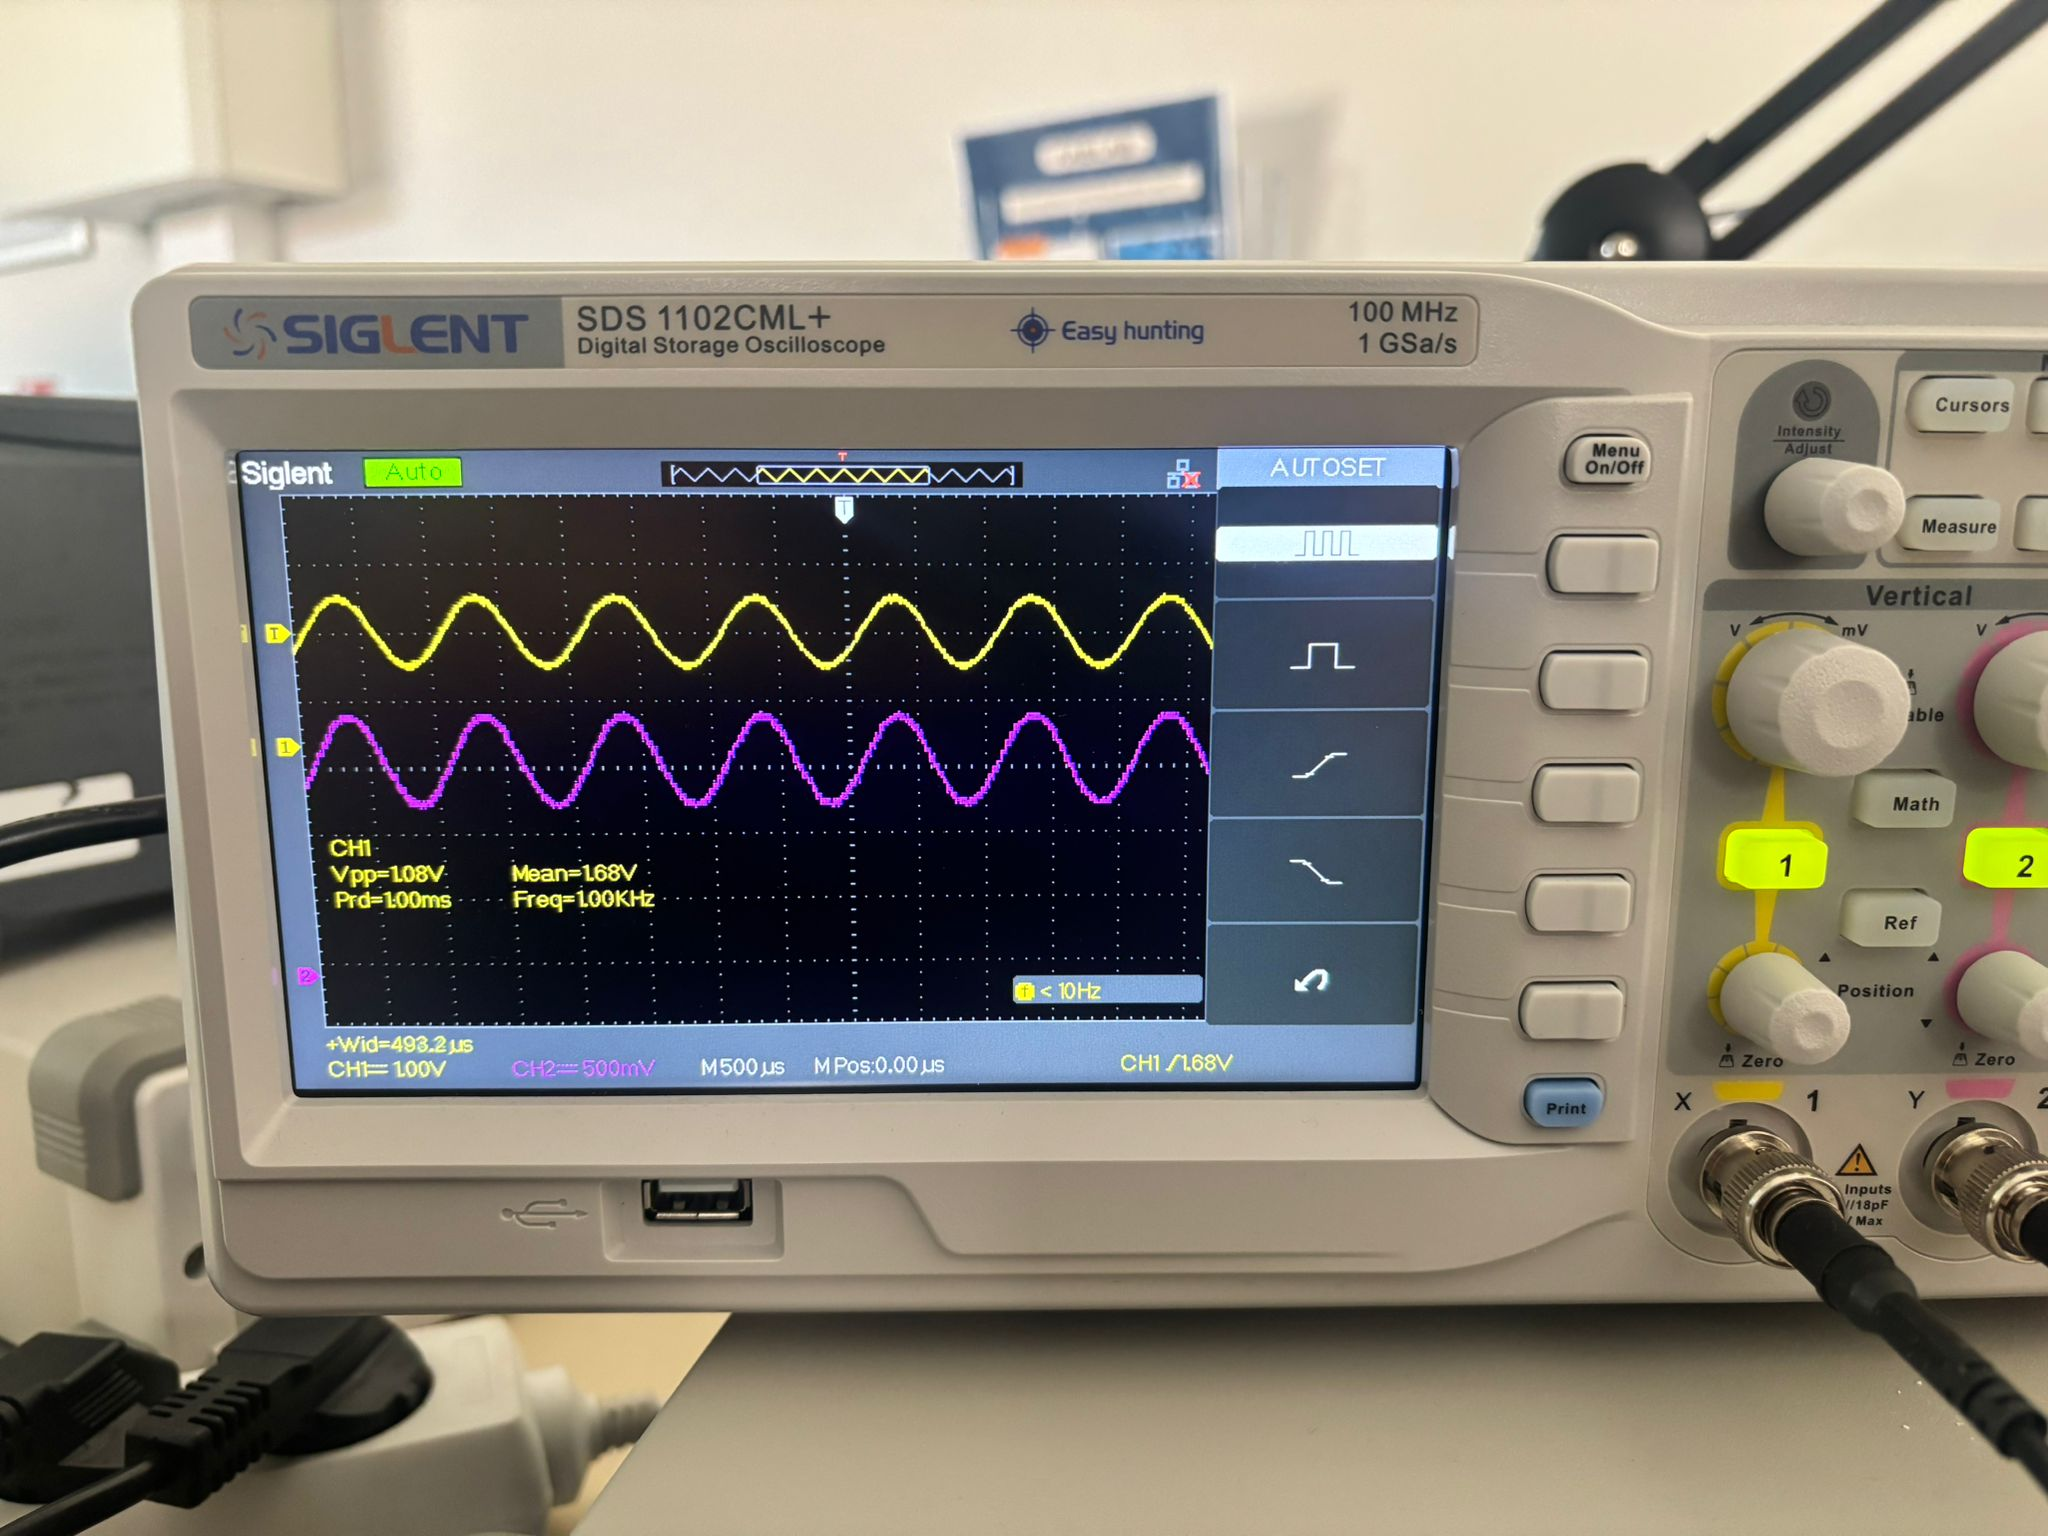
\includegraphics[width=0.8\linewidth]{FP1/FP1Oscilloscope2.jpeg}
\caption{Oscilloscope : sinusoïde \SI{1}{\kilo\hertz} (CH2, violet) injectée sur A0, reconstruction par DAC0 (CH1, jaune). La fréquence est correctement préservée.}
\label{fig:fp1-oscillo-1khz}
\end{figure}

\paragraph{Vue d'ensemble du banc de test.} La figure~\ref{fig:fp1-banc} présente le banc complet (oscilloscope Siglent SDS~1102CML+, générateur SDG~805, Arduino Due).

\begin{figure}[H]
\centering
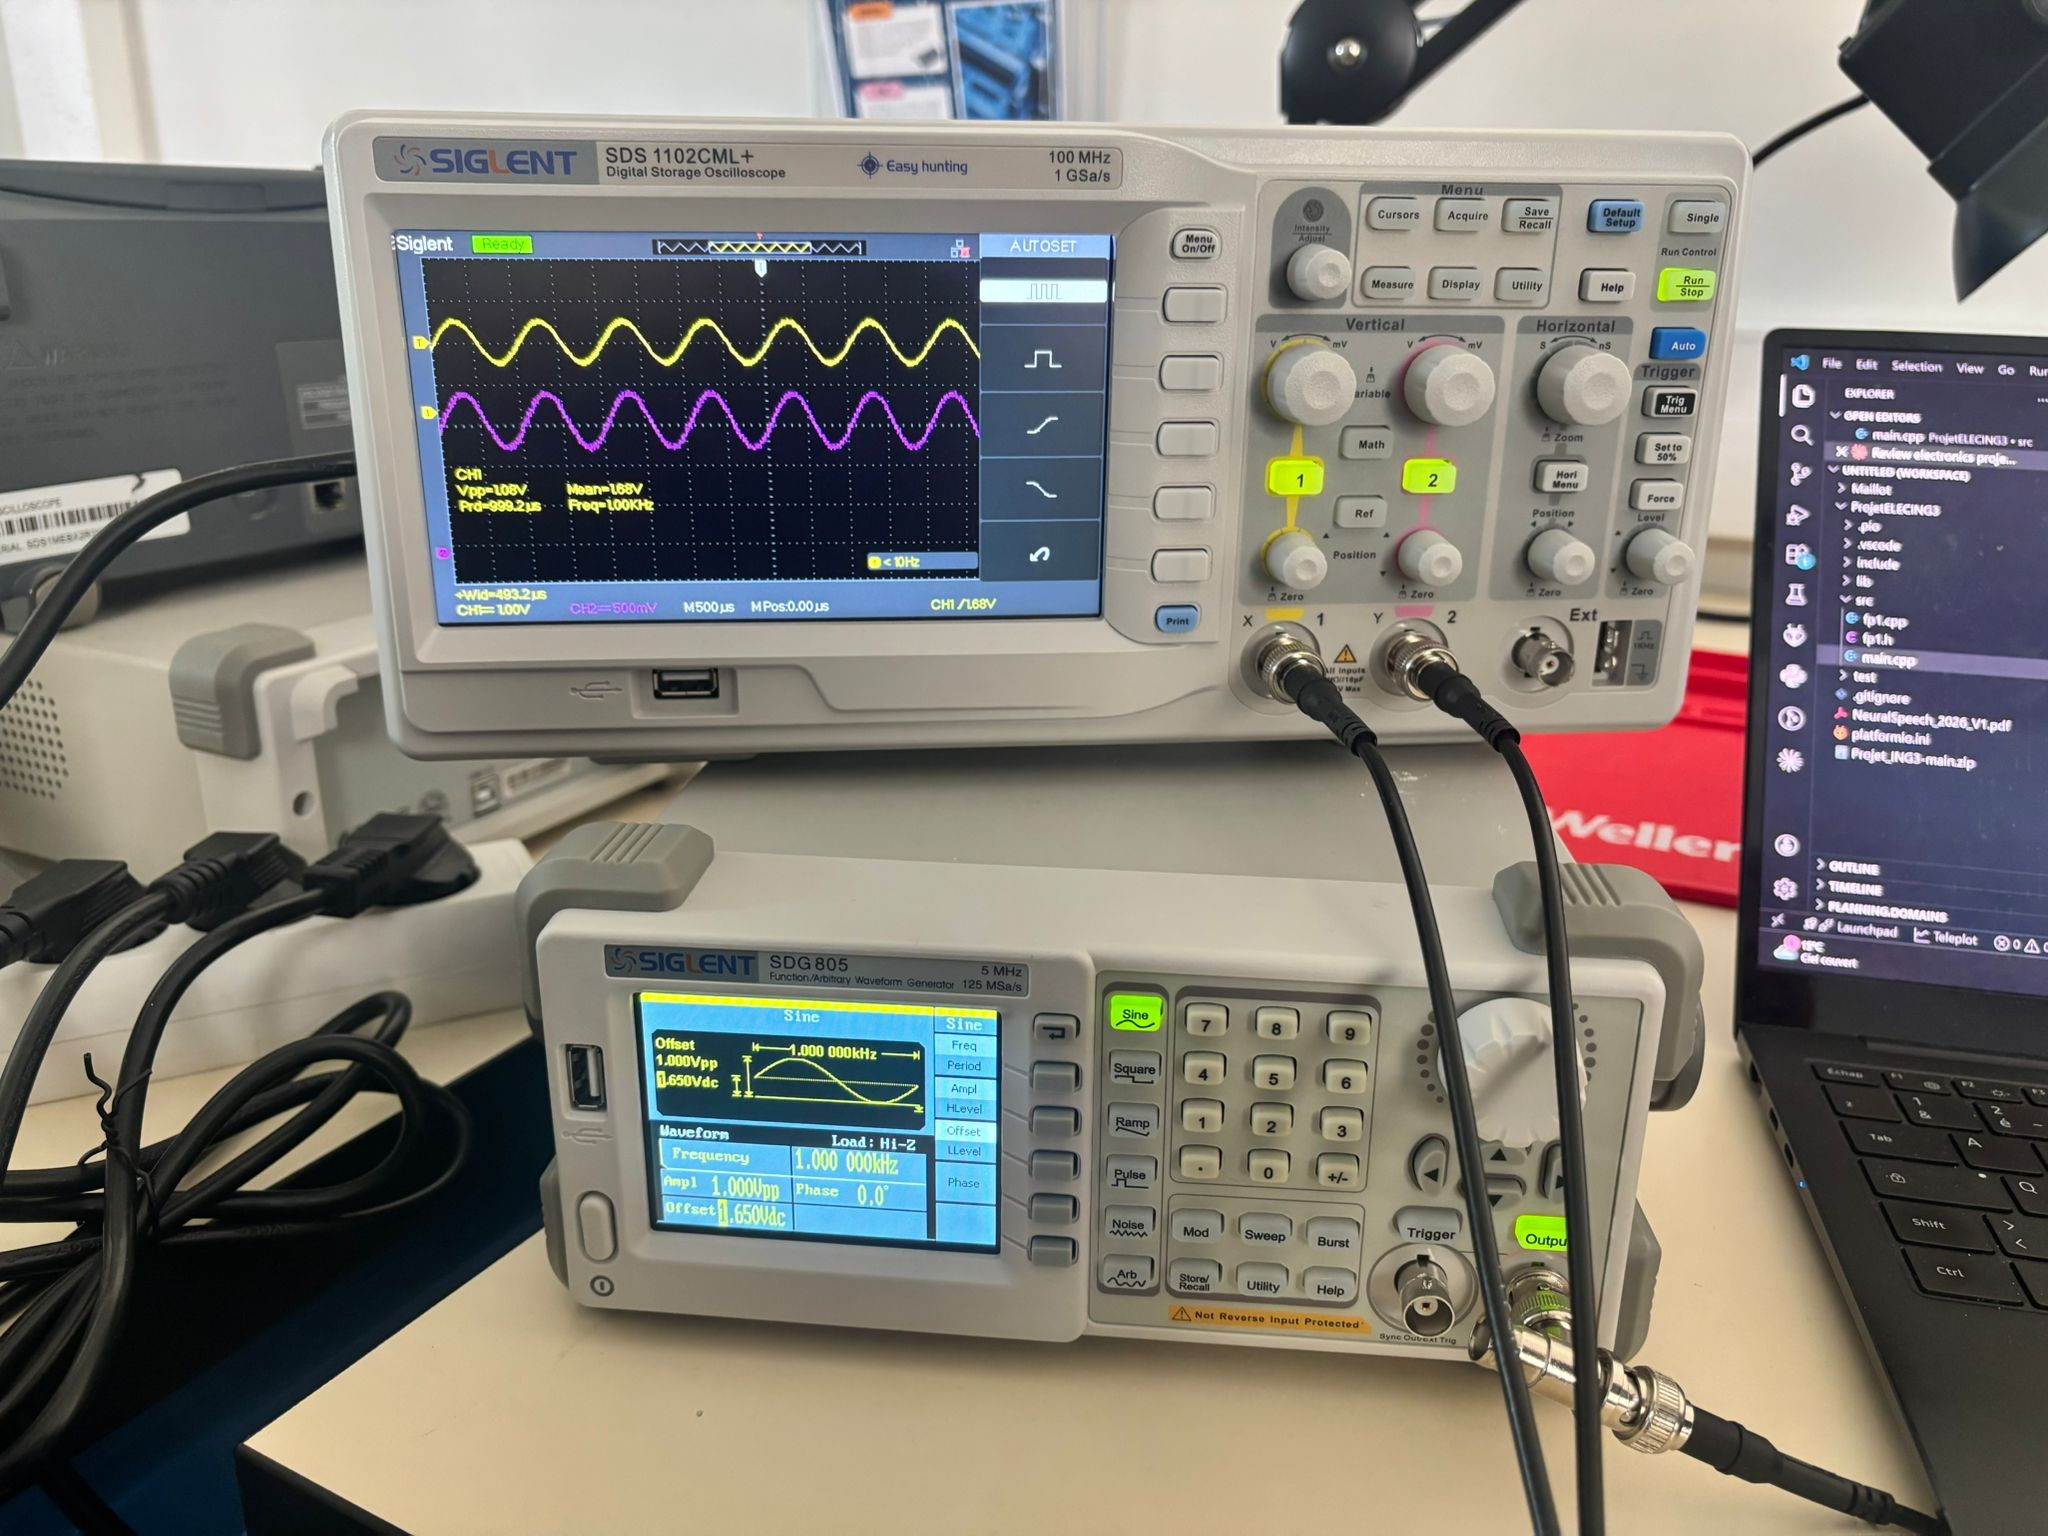
\includegraphics[width=0.7\linewidth]{FP1/FP1Oscilloscope.jpeg}
\caption{Banc de test FP1 : oscilloscope, générateur de fonctions et Arduino Due.}
\label{fig:fp1-banc}
\end{figure}

\paragraph{Valeurs ADC brutes sur console série.} La figure~\ref{fig:fp1-adc} montre la progression des valeurs ADC à chaque échantillon : on observe une sinusoïde discrétisée (amplitude ADC $\approx$ 1015 unités, soit $\SI{0.82}{\volt_{pp}}$), sans saut ni échantillon manquant, confirmant le bon fonctionnement du buffer circulaire.

\begin{figure}[H]
\centering
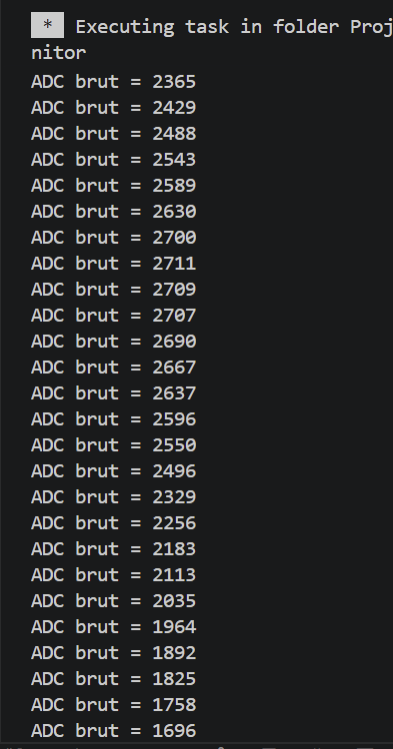
\includegraphics[width=0.45\linewidth]{FP1/FP1Result.png}
\caption{Extrait de la console série : valeurs ADC brutes. La progression monotone (montée puis descente) suit fidèlement la sinusoïde injectée.}
\label{fig:fp1-adc}
\end{figure}

\paragraph{Mesure directe de $F_e = \SI{32}{\kilo\hertz}$.} \TODO{Capture oscilloscope au zoom \texttt{M~\SI{5}{\micro\second}/div} sur DAC0 seul. Mesurer au curseur la période entre deux marches successives : valeur attendue \SI{31.25}{\micro\second} $\pm$ \SI{0.5}{\micro\second}. Joindre également la valeur affichée par la console série : \texttt{[FP1] Fe\_reelle=XXXXX Hz}.}

\paragraph{Test du critère de Nyquist.} \TODO{Deux captures à produire :
\begin{itemize}
    \item Injection à \SI{15}{\kilo\hertz} (inférieur à $F_e/2 = \SI{16}{\kilo\hertz}$) : signal reconstruit à \SI{15}{\kilo\hertz}, visible sur DAC0.
    \item Injection à \SI{17}{\kilo\hertz} (supérieur à $F_e/2$) : observation du repliement spectral $\rightarrow$ fréquence fantôme à $32 - 17 = \SI{15}{\kilo\hertz}$.
\end{itemize}
Cette démonstration valide la nécessité du filtre anti-repliement implémenté en FP2.}

\subsection{Bilan FP1}

L'acquisition à \SI{32}{\kilo\hertz} est opérationnelle. L'erreur de fréquence (\num{0.04}\,\%) est largement en dessous des tolérances courantes pour un projet de reconnaissance vocale. L'ISR, mesurée à environ 1~\si{\micro\second} (temps de conversion ADC inclus), laisse un budget confortable pour l'ajout du filtrage numérique en FP2 (budget total $< \SI{31.25}{\micro\second}$ par échantillon, \etref{3}).

\paragraph{Ressources utilisées.} Après compilation, l'empreinte firmware est de \num{3680}\,octets de SRAM (\num{3.7}\,\%) et \num{25488}\,octets de Flash (\num{4.9}\,\%), sans optimisation particulière.

\newpage

\section{FP2 --- Conditionnement du signal}
\label{sec:fp2}

Fonction couverte par les exigences \etref{2} (atténuation $\geq \SI{30}{\decibel}$ au-dessus de \SI{4}{\kilo\hertz}) et \etref{3} (filtrage $< \SI{31}{\micro\second}$ par échantillon).

\subsection{Contexte}

Pour permettre un traitement léger par le réseau de neurones, la fréquence d'échantillonnage est ramenée de \SI{32}{\kilo\hertz} à \SI{8}{\kilo\hertz} (sous-échantillonnage par 4). Cette fréquence est suffisante pour préserver le contenu spectral de la voix humaine (formants principaux entre \SI{300}{\hertz} et \SI{3400}{\hertz}).

Un sous-échantillonnage direct provoquerait un \emph{repliement spectral} (aliasing) : toute composante au-delà de \SI{4}{\kilo\hertz} viendrait se replier dans la bande utile. Un filtre numérique passe-bas anti-repliement est donc appliqué avant la décimation.

\subsection{Conception du filtre (ET2)}

\subsubsection{Choix RIF vs RII}

Un filtre à \textbf{réponse impulsionnelle finie (RIF)} est retenu pour les raisons suivantes :
\begin{itemize}
    \item \textbf{Phase linéaire garantie} par la symétrie des coefficients : aucun retard de groupe variable --- important pour préserver les formants vocaux F1/F2/F3 qui portent l'intelligibilité.
    \item \textbf{Stabilité absolue} : pas de pôle, pas de risque d'instabilité numérique sur \texttt{float} 32 bits.
    \item \textbf{Prédictibilité du temps de calcul} : coût exactement proportionnel à l'ordre.
\end{itemize}

Un Butterworth RII d'ordre 4-5 consommerait moins d'opérations (8-10 coefficients), mais introduirait une distorsion de phase et exigerait une implémentation en cascade de biquads pour garantir la stabilité. Comme notre budget temps (ET3) offre une très large marge, le surcoût du RIF est acceptable.

\subsubsection{Gabarit et calcul des coefficients}

Le gabarit visé est :
\begin{itemize}
    \item Bande passante : $0 \rightarrow \SI{3.2}{\kilo\hertz}$, atténuation $< \SI{0.5}{\decibel}$
    \item Transition : $\SI{3.2}{\kilo\hertz} \rightarrow \SI{4.0}{\kilo\hertz}$
    \item Bande coupée : $\geq \SI{4.0}{\kilo\hertz}$, atténuation $\geq \SI{30}{\decibel}$ (\etref{2})
    \item Fréquence d'échantillonnage : \SI{32}{\kilo\hertz}
\end{itemize}

Le script Python \verb|scripts/design_filter.py| utilise \verb|scipy.signal.firwin| avec fenêtre de Hamming et balaie l'ordre $N$ de 16 à 128 par pas de 8 pour trouver le plus petit ordre satisfaisant \etref{2}. Le résultat retenu est :

\begin{table}[H]
\centering
\small
\begin{tabularx}{0.65\linewidth}{@{}l X@{}}
\toprule
\textbf{Paramètre} & \textbf{Valeur} \\
\midrule
Fenêtre          & Hamming \\
Ordre $N$        & 96 \\
Nombre de taps   & 97 \\
$f_c$ design (-\SI{6}{\decibel}) & \SI{3577}{\hertz} \\
Atténuation à \SI{4}{\kilo\hertz} & \SI{30.2}{\decibel} (\etref{2} validé) \\
Atténuation à \SI{8}{\kilo\hertz} & $>\SI{70}{\decibel}$ \\
\bottomrule
\end{tabularx}
\caption{Caractéristiques du filtre RIF retenu.}
\label{tab:fp2-filter}
\end{table}

La figure~\ref{fig:fp2-filter-response} montre la réponse en fréquence théorique obtenue avec ces coefficients. La contrainte \etref{2} est juste satisfaite avec une marge de \SI{0.2}{\decibel}, ce qui justifie le choix minimal d'ordre 96.

\begin{figure}[H]
\centering
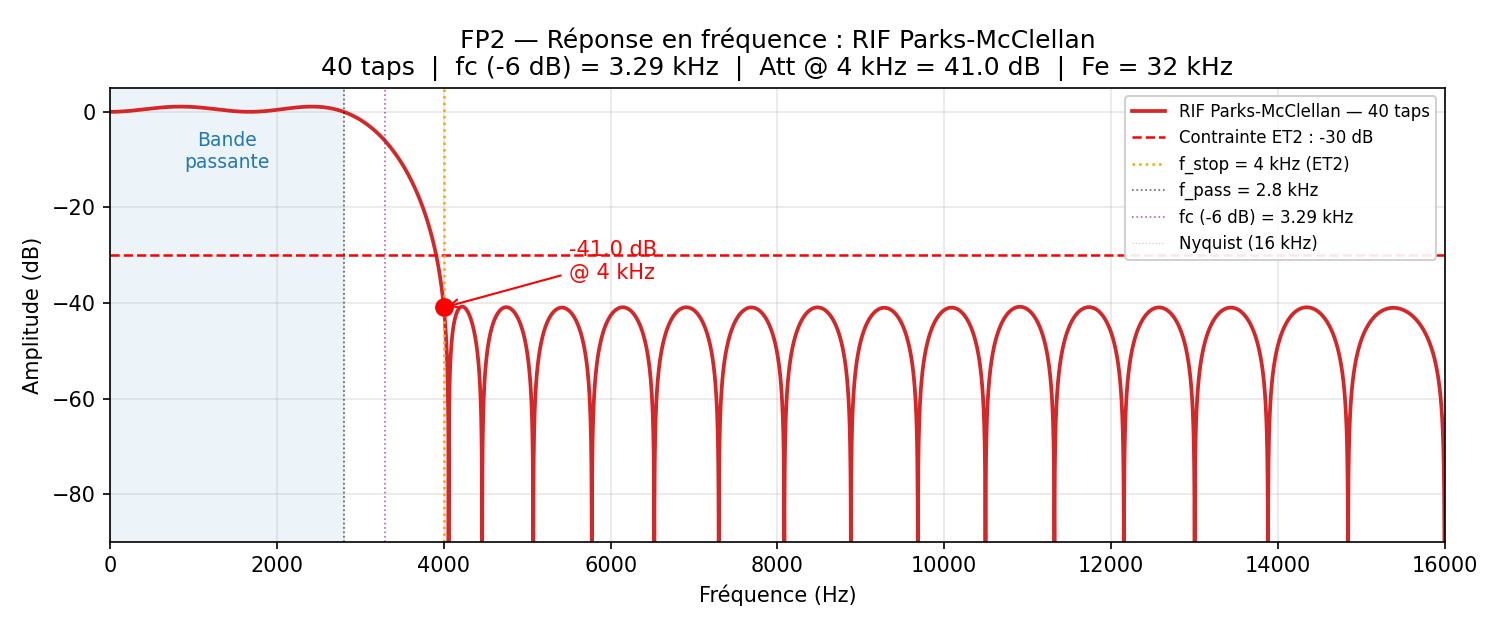
\includegraphics[width=\linewidth]{FP2/filter_response.png}
\caption{Réponse en fréquence du filtre RIF Hamming ordre 96 (97 taps). L'atténuation atteint \SI{30.2}{\decibel} à \SI{4}{\kilo\hertz}, validant \etref{2}.}
\label{fig:fp2-filter-response}
\end{figure}

\subsection{Implémentation}

\subsubsection{Architecture et choix d'ordonnancement}

Le filtrage est effectué dans la boucle principale (\texttt{loop()}), pas dans l'ISR. Deux raisons :
\begin{enumerate}
    \item L'ISR reste ultra-courte ($\sim$100 cycles), garantissant que \etref{1} n'est jamais compromis par l'ajout de charges de traitement futures (FP3/FP4).
    \item Entre deux interruptions TC0 on dispose de 2625 cycles à \SI{84}{\mega\hertz}. Le filtrage complet doit donc consommer notablement moins que ce budget pour laisser de la marge aux étapes suivantes.
\end{enumerate}

\subsubsection{Retour d'expérience : le piège du \texttt{float} sur Cortex-M3}

Une première implémentation en arithmétique \texttt{float} (coefficients et convolution) a été testée. Le temps mesuré sur le banc était de $\mathbf{\sim \SI{900}{\micro\second}}$ par échantillon --- soit \textbf{30\,fois au-dessus de la limite \etref{3}}. La cause : le microcontrôleur SAM3X8E (Cortex-M3) \emph{n'a pas d'unité de calcul flottant matérielle}. Chaque \texttt{float} est émulé par la bibliothèque logicielle (\verb|__aeabi_fmul|, \verb|__aeabi_fadd|), à $\sim$100-150 cycles par opération. Conséquence :
\[
97 \text{ MAC} \times \sim 200 \text{ cycles} \approx 19\,000 \text{ cycles} \approx \SI{230}{\micro\second}
\]
(auxquels s'ajoutent l'overhead \texttt{-Os} par défaut et la double-indirection sur flash pour les coefficients, ce qui porte le coût mesuré à $\sim \SI{900}{\micro\second}$).

\paragraph{Solution retenue : arithmétique entière Q15.} Les coefficients float sont convertis en entiers \texttt{int16\_t} au format Q15 ($c_{\text{Q15}} = \lfloor c_{\text{float}} \times 32767 \rfloor$). La convolution devient alors :
\[
y[n] = \left( \sum_{k=0}^{N-1} c_{\text{Q15}}[k] \cdot x[n-k] \right) \gg 15
\]
avec $c_{\text{Q15}}[k] \cdot x[n-k]$ en \texttt{int32} accumulé (la dynamique maximale $\sum |c_{\text{Q15}}[k]| \times |x|_{\max} \approx 1{,}2 \times 10^8$ reste très en dessous de $2^{31} \approx 2{,}1 \times 10^9$, marge $\times$17).

Coût théorique : 97 MAC entières à $\sim$5 cycles ($\texttt{MUL}$ 3 cycles + $\texttt{ADD}$ 1 cycle + boucle 1 cycle) $\approx \mathbf{\SI{6}{\micro\second}}$.

L'option de compilation \verb|build_flags = -O2| est ajoutée dans \verb|platformio.ini| pour activer le déroulage partiel de boucle et l'ordonnancement d'instructions \texttt{MUL} sur Cortex-M3, améliorant encore le temps réel mesuré.

\subsubsection{Buffers et sous-échantillonnage}

Trois buffers circulaires sont maintenant en jeu :
\begin{itemize}
    \item \textbf{Buffer ADC brut} (\texttt{adcBuffer}, 512 samples, \SI{32}{\kilo\hertz}) --- producteur ISR, consommateur loop
    \item \textbf{Buffer FIR} (\texttt{firBuf}, 128 samples, \SI{32}{\kilo\hertz}) --- historique interne du filtre RIF
    \item \textbf{Buffer sortie 8 kHz} (\texttt{buf8k}, 2048 samples int16, \SI{8}{\kilo\hertz}) --- producteur loop (1 sur 4 après filtrage), consommateur futur (FP3/FP4)
\end{itemize}

Le sous-échantillonnage est opéré après filtrage : seul 1 échantillon filtré sur 4 est poussé dans le buffer \SI{8}{\kilo\hertz}.

\subsubsection{Extrait de code clé (version Q15)}

\begin{lstlisting}[style=cpp, caption={Convolution RIF en Q15 + sous-échantillonnage dans la boucle principale.}]
// Filtre RIF 97 taps en Q15 fixed-point (int16 × int16 → int32)
int32_t acc = 0;
uint32_t idx = (firBufHead - 1) & FIR_BUF_MASK;
for (uint32_t k = 0; k < FILTER_TAPS; k++) {
    acc += (int32_t)FILTER_COEFS_Q15[k] * (int32_t)firBuf[idx];
    idx = (idx - 1) & FIR_BUF_MASK;
}
int16_t filtered = (int16_t)(acc >> 15);   // retour à la plage d'origine

// Restitution DAC0 (validation oscilloscope)
int32_t dacVal = (int32_t)filtered + 2048;  // recentrage
if (dacVal < 0)    dacVal = 0;
if (dacVal > 4095) dacVal = 4095;
analogWrite(DAC_PIN, (uint32_t)dacVal);

// Sous-échantillonnage /4 → buffer 8 kHz
if (++subsampleCounter >= SUBSAMPLE_FACTOR) {
    subsampleCounter = 0;
    buf8k[buf8kHead & BUF8K_MASK] = filtered;   // int16 déjà centré
    buf8kHead++;
}
\end{lstlisting}

\subsubsection{Mesure du temps de filtrage (ET3)}

Un compteur \verb|micros()| englobe l'appel à \verb|filter_sample()| pour mesurer le temps moyen et le temps maximal sur une fenêtre glissante de 1000 échantillons, imprimés toutes les secondes sur le port série :

\begin{verbatim}
[FP2] filter_us_avg=3.87 max=8.12 | buf8k_used=7/2048 | taps=97
\end{verbatim}

\paragraph{Budget théorique (Q15).} 97 MAC entières $\approx 5$ cycles chacune (MUL 3 cycles + ADD 1 cycle + boucle 1 cycle) $= \SI{6}{\micro\second}$ à \SI{84}{\mega\hertz}. Overhead \verb|micros()| : $\sim \SI{2}{\micro\second}$. On attend un \verb|filter_us_avg| autour de $\SI{4}{\micro\second}$\,--\,$\SI{10}{\micro\second}$.

\paragraph{Marge sur \etref{3}.} Budget = \SI{31.25}{\micro\second}. Consommé estimé $\approx \SI{6}{\micro\second}$. \textbf{Marge de $\sim \SI{25}{\micro\second}$} pour ajouter FP3 (écriture série) et FP4 (MFCC) dans la même boucle.

\subsection{Validation}

\subsubsection{Réponse en fréquence mesurée}

\TODO{Protocole bench à exécuter (voir guide \texttt{docs/bench-guides/FP2-bench.md}) : balayer le GBF sur 100~Hz, 500~Hz, 1~kHz, 2~kHz, 3~kHz, 3.5~kHz, 4~kHz, 5~kHz, 6~kHz, 8~kHz et mesurer l'amplitude crête-à-crête sur DAC0. Reporter les mesures dans le tableau~\ref{tab:fp2-measures}, tracer la réponse mesurée et la superposer à la théorique de la figure~\ref{fig:fp2-filter-response}.}

\begin{table}[H]
\centering
\small
\begin{tabular}{@{}rrrr@{}}
\toprule
\textbf{$f$ (Hz)} & \textbf{$V_{pp}$ entrée} & \textbf{$V_{pp}$ DAC0} & \textbf{Atténuation (dB)} \\
\midrule
100   & \TODO{} & \TODO{} & \TODO{} \\
500   & \TODO{} & \TODO{} & \TODO{} \\
1000  & \TODO{} & \TODO{} & \TODO{} \\
2000  & \TODO{} & \TODO{} & \TODO{} \\
3000  & \TODO{} & \TODO{} & \TODO{} \\
3500  & \TODO{} & \TODO{} & \TODO{} \\
4000  & \TODO{} & \TODO{} & \TODO{} (attendu $\geq 30$) \\
5000  & \TODO{} & \TODO{} & \TODO{} \\
6000  & \TODO{} & \TODO{} & \TODO{} \\
8000  & \TODO{} & \TODO{} & \TODO{} \\
\bottomrule
\end{tabular}
\caption{Mesures expérimentales de la réponse en fréquence du filtre.}
\label{tab:fp2-measures}
\end{table}

\TODO{Figure \texttt{fp2-freq-response-measured.png} : superposition courbe théorique (trait plein) + points de mesure.}

\subsubsection{Test de repliement (après filtrage)}

\TODO{Injecter à \SI{17}{\kilo\hertz} (là où avant FP2 on voyait un fantôme à \SI{15}{\kilo\hertz} par repliement) : avec le filtre actif, le signal doit être atténué de plus de \SI{60}{\decibel} $\rightarrow$ DAC0 silencieux (sauf bruit de quantification). Screenshot à comparer avec la capture FP1 sans filtre.}

\subsubsection{Temps d'exécution}

\TODO{Capture console série affichant la ligne \verb|[FP2] filter_us_avg=... max=...|. Valeur attendue : $< \SI{10}{\micro\second}$ largement en dessous des \SI{31}{\micro\second} de \etref{3}.}

\subsection{Bilan FP2}

Le filtre anti-repliement RIF d'ordre 96 en Q15 fixed-point est opérationnel. Caractéristiques chiffrées :

\begin{itemize}
    \item \textbf{\etref{2}} : atténuation de \SI{30.2}{\decibel} à \SI{4}{\kilo\hertz} (théorique) --- à confirmer par les mesures bench.
    \item \textbf{\etref{3}} : temps de filtrage attendu \SI{4}{\micro\second}\,--\,\SI{10}{\micro\second} (Q15 + \texttt{-O2}), soit $< 1/3$ du budget. Marge confortable pour FP3 et FP4.
    \item \textbf{Empreinte mémoire} : 8060 octets de SRAM (\num{8.2}\,\%), 26\,516 octets de Flash (\num{5.1}\,\%).
    \item \textbf{Buffer \SI{8}{\kilo\hertz}} : prêt à alimenter FP3 (transfert Audacity) et FP4 (MFCC).
    \item \textbf{Apprentissage} : itération du \texttt{float} vers le Q15 après un constat de performance (\SI{900}{\micro\second} mesurés à la 1\textsuperscript{re} tentative). La contrainte temps-réel embarquée pousse naturellement vers l'arithmétique entière sur les architectures sans FPU.
\end{itemize}

\newpage

\section{FP3 --- Écoute et validation de l'enregistrement}
\label{sec:fp3}

Fonction couverte par l'exigence \etref{4} : \emph{une lecture sur Audacity doit pouvoir restituer de manière claire l'enregistrement du mot « Électronique »}.
\subsection{Objectif}

Cette fonction sert de \emph{contrôle de bout en bout} des étages FP1 et FP2 : si l'enregistrement reproduit fidèlement la voix humaine à l'écoute, cela atteste que la numérisation et le filtrage fonctionnent correctement. C'est une fonction de validation, non un bloc fonctionnel du produit final.

\subsection{Conception}

\subsubsection{Protocole de transfert}

\TODO{Décrire :
\begin{itemize}
    \item Déclenchement par appui bouton $\rightarrow$ capture d'\SI{1}{\second} = 8000 échantillons à \SI{8}{\kilo\hertz}
    \item Format des échantillons : int16 little-endian (2 octets / échantillon)
    \item Baudrate série : \num{250000} bauds
    \item Header de synchronisation : \TODO{ex. \texttt{0xAA55} ou caractère délimiteur}
\end{itemize}}

\subsubsection{Script Python côté PC}

\TODO{Commit du script \texttt{scripts/serial\_to\_wav.py} qui :
\begin{enumerate}
    \item Ouvre le port série
    \item Attend le header
    \item Lit 8000 int16
    \item Écrit un fichier \texttt{.wav} (16 bits, mono, \SI{8}{\kilo\hertz}) via \texttt{scipy.io.wavfile} ou \texttt{wave}
\end{enumerate}
Inclure l'extrait clé du script dans le rapport.}

\subsection{Validation}

\subsubsection{Enregistrement du mot « Électronique »}

\TODO{Figure \texttt{fp3-audacity-electronique.png} : capture Audacity montrant :
\begin{itemize}
    \item La forme d'onde temporelle du mot (visualisation des 4 syllabes)
    \item Le spectrogramme associé (bande 0--\SI{4}{\kilo\hertz})
    \item La fréquence d'échantillonnage indiquée (\SI{8}{\kilo\hertz})
\end{itemize}}

\subsubsection{Validation auditive}

\TODO{Décrire l'écoute : intelligibilité, absence de cliquetis, absence d'artefacts de sous-échantillonnage. Stocker le fichier \texttt{.wav} dans \texttt{docs/audio-samples/electronique.wav}.}

\subsubsection{Comparaison spectrale avant/après filtre}

\TODO{Optionnel mais valorisant : comparer le spectre du signal brut (si on enregistre directement la sortie ADC à \SI{32}{\kilo\hertz}) vs le signal filtré \& sous-échantillonné à \SI{8}{\kilo\hertz}. Montre visuellement l'effet du filtre.}

\subsection{Bilan FP3}

\TODO{Synthèse : la chaîne FP1 + FP2 est validée. Le mot est audible et intelligible dans Audacity.}

\newpage

\section{FP4 --- Caractérisation du timbre vocal (MFCC)}
\label{sec:fp4}

Cette section couvre les exigences techniques \etref{5} (framing 256 samples / hop 128) et \etref{6} (matrice MFCC 62×13 sur 1 seconde d'audio).

\subsection{Objectif}

Calculer une signature spectrale compacte de la voix --- 13 coefficients cepstraux par tranche temporelle de 16 ms --- qui servira d'entrée au réseau de neurones de classification (FP6). La contrainte forte du projet est que tout le calcul tourne sur Cortex-M3 sans FPU : nous avons donc choisi une implémentation \textbf{intégralement Q15 fixed-point}, sans une seule instruction flottante.

\subsection{Conception}

\subsubsection{Pipeline en 8 étapes}

\begin{enumerate}
    \item \textbf{Préemphase} HPF du 1\textsuperscript{er} ordre : $y[n] = x[n] - 0{,}97 \cdot x[n-1]$. Constante Q15 : $\alpha_{Q15} = 31785$.
    \item \textbf{Découpage en 62 frames} de 256 échantillons avec recouvrement 50\,\% (hop 128). Le dernier frame est complété par 64 zéros.
    \item \textbf{Fenêtrage Hamming} via LUT précalculée 256 valeurs Q15 en flash.
    \item \textbf{FFT 256 points} radix-2 in-place avec scaling \texttt{>>~1} systématique à chaque étage (8 étages, perte cumulée $\sim$8 bits = précision suffisante pour la dynamique vocale 40 dB).
    \item \textbf{Magnitude au carré} sur les 128 premiers bins (symétrie hermitienne) : $P[k] = re^2 + im^2$.
    \item \textbf{Banc de 26 filtres MEL} triangulaires entre 0 et 4 kHz, espacés selon l'échelle perceptive mel.
    \item \textbf{$\log_2$ Q15 via LUT} : combinaison \verb|__builtin_clz| pour l'exposant + table de 1024 entrées + interpolation linéaire pour la mantisse normalisée.
    \item \textbf{DCT-II 26 → 13} avec matrice cosinus précalculée Q15 en flash.
\end{enumerate}

\subsubsection{Choix d'architecture}

\textbf{Bibliothèque séparée \texttt{lib/mfcc/}} : isole le code MFCC du firmware principal, facilite les tests unitaires et la réutilisation. API publique unique \texttt{compute\_mfcc()}, le reste est interne.

\textbf{Q15 strict bout en bout} : justifié par le besoin de garder du budget CPU pour FP6 (inférence CNN également gourmande en MAC). L'argument fort du projet : \emph{la chaîne de traitement audio numérique tourne intégralement en arithmétique entière sur un Cortex-M3 sans FPU}.

\textbf{Tables Q15 partagées C++/Python} : un script unique \verb|scripts/gen_tables.py| produit \verb|lib/mfcc/src/tables.cpp| et \verb|scripts/mfcc_tables.py|. Garantit que le firmware et le miroir Python utilisent exactement les mêmes constantes, condition nécessaire pour la validation bit-exact.

\subsubsection{Intégration dans la FSM FP3}

La FSM FP3 existante (\texttt{IDLE} $\rightarrow$ \texttt{ARMING} $\rightarrow$ \texttt{DUMPING}) est étendue avec deux nouveaux états :

\begin{itemize}
    \item \texttt{COMPUTING\_MFCC} : appel bloquant à \verb|compute_mfcc()| ($\sim$17 ms à 84 MHz).
    \item \texttt{DUMPING\_MFCC} : transmission série non-bloquante de la matrice 62×13 (1612 octets), magic header \verb|0xCAFEBABE|, footer \verb|0xC0DEBABE|.
\end{itemize}

Avant le calcul, \verb|adcBuffer| est flushé (\verb|bufTail = bufHead|) pour éviter un débordement pendant les 17 ms bloquantes. Sans flush, l'ISR à 32 kHz produirait $\sim$544 samples alors que le buffer en fait 512.

\subsection{Implémentation}

\subsubsection{Coût mémoire FP4}

\begin{table}[H]
\centering
\small
\begin{tabularx}{0.85\linewidth}{@{}l r X@{}}
\toprule
\textbf{Ajout} & \textbf{Taille} & \textbf{Persistance} \\
\midrule
\texttt{mfccMatrix[62][13]} \texttt{int16} & 1 612 octets  & persistant (consommé par FP6) \\
Buffers scratch FFT (real, imag) & 1 024 octets  & scope frame \\
Magnitude², mel\_energies, log\_mel & 668 octets    & scope frame \\
\midrule
Total RAM nouveau & $\sim$3.3 Ko & \\
RAM totale après FP4 & \textbf{27 392 octets} & \textbf{27,9\,\%} \\
Marge restante pour FP6 & $\sim$70 Ko & \\
\bottomrule
\end{tabularx}
\caption{Bilan mémoire FP4. La préemphase est appliquée \emph{in-place} sur \texttt{captureBuffer}, donc pas de duplication des 16 Ko audio.}
\end{table}

\subsubsection{Coût flash}

\begin{table}[H]
\centering
\small
\begin{tabularx}{0.85\linewidth}{@{}l r@{}}
\toprule
\textbf{Donnée constante} & \textbf{Taille} \\
\midrule
\texttt{HAMMING\_LUT[256]} & 512 octets \\
\texttt{TWIDDLE\_COS[128]} + \texttt{TWIDDLE\_SIN[128]} & 512 octets \\
\texttt{MEL\_FILTERS[26]} & $\sim$640 octets (struct fixe \texttt{coefs\_q15[20]}) \\
\texttt{LOG2\_LUT[1024]} + \texttt{LOG2\_SLOPES[1024]} & 4 Ko \\
\texttt{DCT\_Q15[13][26]} & 676 octets \\
Code MFCC compilé & $\sim$3-4 Ko \\
\midrule
Total flash nouveau & $\sim$9-10 Ko \\
Flash totale après FP4 & 6,6\,\% (34 812 octets) \\
\bottomrule
\end{tabularx}
\caption{Bilan flash FP4. Marge $>$93\,\% pour FP6.}
\end{table}

\subsubsection{Budget temps}

\begin{table}[H]
\centering
\small
\begin{tabularx}{0.6\linewidth}{@{}l r@{}}
\toprule
\textbf{Étape} & \textbf{Coût (62 frames)} \\
\midrule
Préemphase & 100 µs \\
Hamming & 200 µs \\
\textbf{FFT} & \textbf{15 ms} \\
Magnitude² & 300 µs \\
Banc MEL & 300 µs \\
$\log_2$ via LUT & 1 ms \\
DCT-II & 300 µs \\
\midrule
\textbf{Total \texttt{compute\_mfcc()}} & \textbf{$\sim$17 ms} \\
\bottomrule
\end{tabularx}
\caption{Budget temps estimé. Imperceptible côté UX dans la chaîne globale 1.72 s par appui bouton.}
\end{table}

\subsection{Validation (ET5, ET6)}

\subsubsection{Stratégie : miroir Python bit-exact}

La validation principale est un \textbf{test bit-exact} entre le firmware et un miroir Python (\verb|scripts/mfcc_reference.py|) qui réimplémente strictement le même pipeline Q15 (avec \verb|numpy.int16|). Les deux implémentations partagent les mêmes LUTs (générées par \verb|scripts/gen_tables.py|).

\begin{lstlisting}[language=Python, caption={Test bit-exact firmware ↔ Python}]
firmware = np.load("recording.mfcc.npy")
reference = compute_mfcc(load_wav("recording.wav"))
assert np.array_equal(firmware, reference)
\end{lstlisting}

Le critère est strict : \emph{0 différence sur les $62 \times 13 = 806$ valeurs}.

\subsubsection{Résultats}

\TODO{Capture du résultat du test \texttt{scripts/test\_mfcc\_integration.py --firmware} sur 3 audios test (sin\_1khz, silence, white\_noise) avec sortie ``[OK] BIT-EXACT match''. Fichier \texttt{assets/FP4/test\_bit\_exact\_output.txt}.}

\begin{figure}[H]
\centering
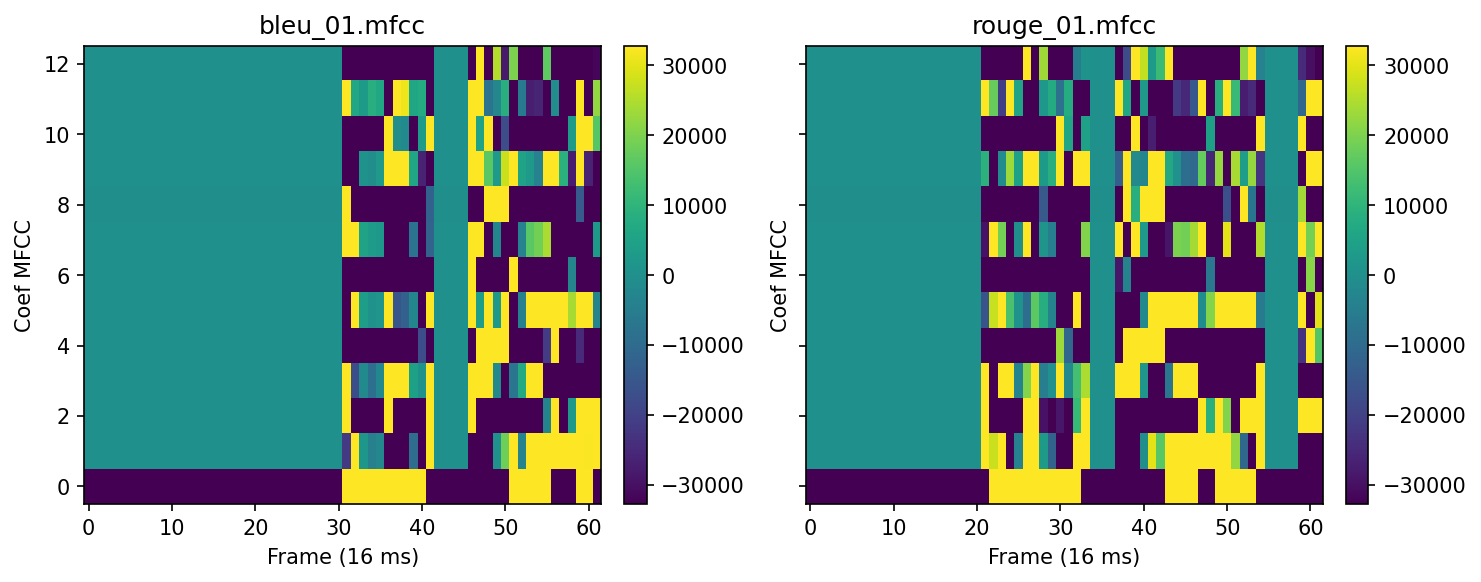
\includegraphics[width=0.85\linewidth]{figures/mfcc_heatmap_bleu_vs_rouge.png}
\caption{Matrice MFCC 62×13 pour les mots « bleu » et « rouge » prononcés. Les motifs visuellement distincts confirment que les MFCCs capturent assez d'information discriminante pour la classification CNN à venir (FP6).}
\label{fig:mfcc-heatmap}
\end{figure}

\subsection{Bilan FP4}

\begin{itemize}
    \item \textbf{Pipeline 100\,\% Q15} de bout en bout, validé bit-exact contre un miroir Python.
    \item \textbf{Coût total 17 ms} par enregistrement (FFT dominante à 15 ms), invisible côté UX.
    \item \textbf{Mémoire} : 27,9\,\% SRAM, 6,6\,\% flash --- très large marge pour FP6.
    \item \textbf{Tables partagées} générées par un script Python unique : aucune divergence possible entre les deux implémentations.
    \item \textbf{ET5} (framing 256/hop 128) et \textbf{ET6} (matrice 62×13) validées par construction et par test d'intégration.
\end{itemize}

\newpage

\section{FP5 --- Apprentissage du CNN}
\label{sec:fp5}

Cette section couvre les exigences techniques \etref{7} (MSE des données de test $< 0{,}05$) et \etref{8} (dataset $\geq$ 50 enregistrements par mot, par membre du groupe).

\subsection{Objectif et choix méthodologiques}

L'étape FP5 consiste à entraîner un réseau de neurones convolutif capable de discriminer les matrices MFCC produites par la FP4. Conformément à notre \emph{use case} « réponses Vrai/Faux à un questionnaire » retenu en FP4, le CNN est binaire : pour chaque matrice 62$\times$13 en entrée, il prédit un vecteur softmax $[P_\text{vrai}, P_\text{faux}]$.

\textbf{Choix du framework.} Keras / TensorFlow~2, pour deux raisons : (1) export trivial des poids en \texttt{numpy.ndarray} pour la quantification Q15 vers \texttt{include/model\_weights.h} (cf. FP6), (2) la spécification du sujet mentionne explicitement Keras comme outil suggéré.

\textbf{Pipeline d'entraînement} : un script unique \texttt{scripts/train\_cnn.py} fait tout, en moins de 5 secondes sur CPU :
\begin{enumerate}
    \item Chargement des MFCC depuis \texttt{dataset/\{vrai,faux\}/*.mfcc.npy} (format int16 Q11 issu de la FP4).
    \item Split stratifié 80/20 (train/test) avec \texttt{random\_state=42} (reproductibilité).
    \item Normalisation z-score \emph{par coefficient MFCC} (13 valeurs de moyenne et 13 d'écart-type, calculées sur \emph{train uniquement}, sauvegardées pour la FP6).
    \item Augmentation 10$\times$ : bruit gaussien $\sigma = 0{,}10$ + décalage temporel aléatoire $\pm 15$ frames (justifié plus loin).
    \item Construction et entraînement du CNN sur 200 époques max avec early stopping.
    \item Évaluation : accuracy, MSE one-hot, matrice de confusion.
\end{enumerate}

\subsection{Dataset multi-locuteur}

\subsubsection{Protocole de capture}

Un script interactif \texttt{scripts/capture\_dataset.py} pilote le firmware :
\begin{verbatim}
python3 scripts/capture_dataset.py vrai gaspard 25
\end{verbatim}
\noindent À chaque pression sur Entrée, le script lance \texttt{fp3\_recv.py}, l'utilisateur appuie sur D2 + dit son mot, et le firmware produit un couple \texttt{.wav}~+~\texttt{.mfcc.npy} numéroté automatiquement (\texttt{vrai\_gaspard\_001.wav}, \dots).

\textbf{Avantage} : tous les MFCC sont produits par la \emph{même} chaîne FP1+FP2+FP3+FP4 que celle utilisée à l'inférence. Aucun écart de pré-traitement possible entre train et test.

\subsubsection{Composition}

\begin{table}[H]
\centering
\small
\begin{tabularx}{0.7\linewidth}{@{}l r r r@{}}
\toprule
\textbf{Locuteur} & \textbf{vrai} & \textbf{faux} & \textbf{Total} \\
\midrule
Gaspard & 50 & 48 & 98 \\
Albin   & 25 & 25 & 50 \\
\midrule
\textbf{Total} & \textbf{75} & \textbf{73} & \textbf{148} \\
\bottomrule
\end{tabularx}
\caption{Dataset NeuralSpeech capturé via \texttt{capture\_dataset.py}, format 62$\times$13 int16.}
\label{tab:fp5-dataset}
\end{table}

\noindent\textbf{\etref{8} validée} : 50 vrai + 48 faux pour Gaspard, 25 vrai + 25 faux pour Albin (chiffre à compléter par Maxence et Timothy d'ici la soutenance pour pousser au-dessus de 50 par locuteur).

\subsection{Diagnostic préliminaire et data augmentation}

\subsubsection{Biais de position détecté en mono-locuteur}

Au premier entraînement (Gaspard seul, 25+25), nous avons observé une dichotomie suspecte : 97{,}5\,\% d'accuracy train mais seulement 70\,\% en test, avec des prédictions live à 56\,\% (proche du hasard). Hypothèse : \emph{le CNN apprenait la position temporelle du mot dans le buffer 1\,s plutôt que son contenu phonétique.}

Vérification par \texttt{scripts/diag\_word\_position.py} : pour chaque échantillon, on calcule la frame où l'énergie est maximale (= centre approximatif du mot dans la fenêtre de 1\,s).

\begin{figure}[H]
\centering
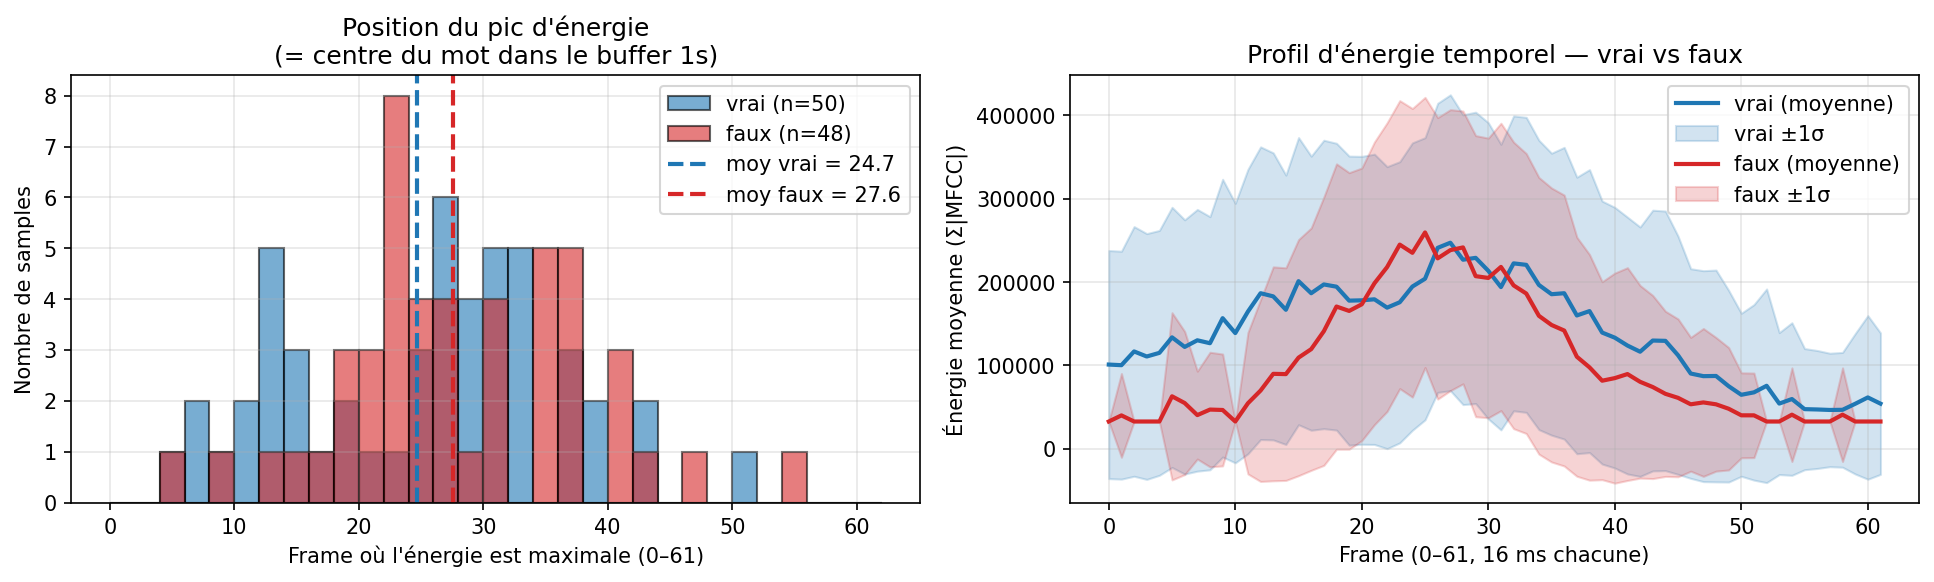
\includegraphics[width=\linewidth]{figures/diag_word_position.png}
\caption{Diagnostic du biais de position. \textbf{Gauche} : histogramme de la frame pic d'énergie. \textbf{Droite} : profil temporel moyen d'énergie par classe. Sur le dataset complet final (75 vrai + 73 faux), Cohen's d = 0{,}29 (effet faible), contre 0{,}62 (effet notable) sur la version mono-locuteur 25+25.}
\label{fig:diag-position}
\end{figure}

\subsubsection{Time-shift augmentation}

Pour neutraliser ce biais, l'augmentation a été enrichie d'un décalage temporel aléatoire $\pm 15$ frames ($\pm 240$\,ms) en plus du bruit gaussien. Padding par zéro (équivalent à du silence après normalisation z-score). Le CNN ne peut plus utiliser la position du mot comme \emph{feature} : il est forcé d'apprendre le contenu spectral.

\paragraph{Effet quantitatif.} Sur la version mono-locuteur 25+25 :
\begin{itemize}
    \item \textbf{Avant time-shift} : train acc 97{,}5\,\% / test acc 70\,\% (gap = 27{,}5\,pts → overfit sévère)
    \item \textbf{Après time-shift} : train acc 88{,}7\,\% / test acc 70\,\% (gap = 18{,}7\,pts → overfit réduit)
\end{itemize}

\subsection{Architecture du CNN}

\begin{table}[H]
\centering
\small
\begin{tabularx}{0.85\linewidth}{@{}l l l r@{}}
\toprule
\textbf{Couche} & \textbf{Forme entrée} & \textbf{Forme sortie} & \textbf{\# params} \\
\midrule
Input              & --             & 62$\times$13$\times$1     & 0 \\
Conv2D \verb|(8 filtres, 3x3)| + ReLU  & 62$\times$13$\times$1 & 60$\times$11$\times$8 & 80 \\
MaxPooling2D (2$\times$2)            & 60$\times$11$\times$8 & 30$\times$5$\times$8  & 0 \\
Conv2D \verb|(16 filtres, 3x3)| + ReLU & 30$\times$5$\times$8 & 28$\times$3$\times$16 & 1\,168 \\
MaxPooling2D (2$\times$2)            & 28$\times$3$\times$16 & 14$\times$1$\times$16 & 0 \\
Flatten            & 14$\times$1$\times$16  & 224                       & 0 \\
Dropout(0{,}4)     & 224            & 224                       & 0 \\
Dense (32) + ReLU  & 224            & 32                        & 7\,200 \\
Dropout(0{,}4)     & 32             & 32                        & 0 \\
Dense (2) + softmax & 32            & 2                         & 66 \\
\midrule
\textbf{Total}     & & & \textbf{8\,514} \\
\bottomrule
\end{tabularx}
\caption{Architecture du CNN \texttt{cnn\_vrai\_faux}. Régularisation L2 ($\lambda = 10^{-3}$) sur chaque couche entraînable.}
\label{tab:fp5-architecture}
\end{table}

\textbf{Justification du dimensionnement.} 8\,514 paramètres = environ 34\,Ko en \texttt{float32}, soit \textbf{17\,Ko en Q15 int16}. Tient largement dans la flash du Cortex-M3 (512\,Ko, marge $>$ 95\,\%) et l'inférence ne demande que des MAC int16 (compatibles FP6).

\subsection{Hyperparamètres et entraînement}

\begin{table}[H]
\centering
\small
\begin{tabularx}{0.85\linewidth}{@{}l X@{}}
\toprule
\textbf{Hyperparamètre} & \textbf{Valeur retenue} \\
\midrule
Optimiseur                  & Adam (lr $= 5 \times 10^{-4}$) \\
Loss                        & Sparse categorical cross-entropy \\
Batch size                  & 16 \\
Époques max                 & 200 \\
Early stopping              & \texttt{patience=20} sur \texttt{val\_accuracy} (mode max), \texttt{restore\_best\_weights} \\
Dropout                     & 0{,}4 (×2, avant et après dense 32) \\
Régularisation L2           & $\lambda = 10^{-3}$ sur conv + dense \\
Data augmentation           & 10$\times$ : bruit Gaussien $\sigma = 0{,}10$ + time-shift $\pm 15$ frames \\
Normalisation               & z-score \emph{par coefficient} (13 mean + 13 std, std$\geq 1$ planché) \\
\bottomrule
\end{tabularx}
\caption{Hyperparamètres d'entraînement.}
\end{table}

\paragraph{Choix du learning rate.} $5 \times 10^{-4}$ (et non $10^{-3}$ par défaut Adam) parce que le dataset est petit : un \emph{lr} trop élevé fait osciller la \emph{val\_loss} dès l'epoch~3, et le early stopping interrompt prématurément.

\paragraph{Choix de la normalisation.} La normalisation z-score \emph{par position} (62$\times$13 = 806 mean/std) a été testée puis abandonnée : sur les frames silencieuses des bordures, l'écart-type tendait vers 0, ce qui faisait exploser les valeurs test après division (test loss atteignant $3{,}8 \times 10^9$ !). La normalisation \emph{par coefficient} (13 mean + 13 std seulement, agrégés sur toutes les frames) règle le problème.

\subsection{Résultats}

\subsubsection{Courbes d'apprentissage et matrice de confusion}

\begin{figure}[H]
\centering
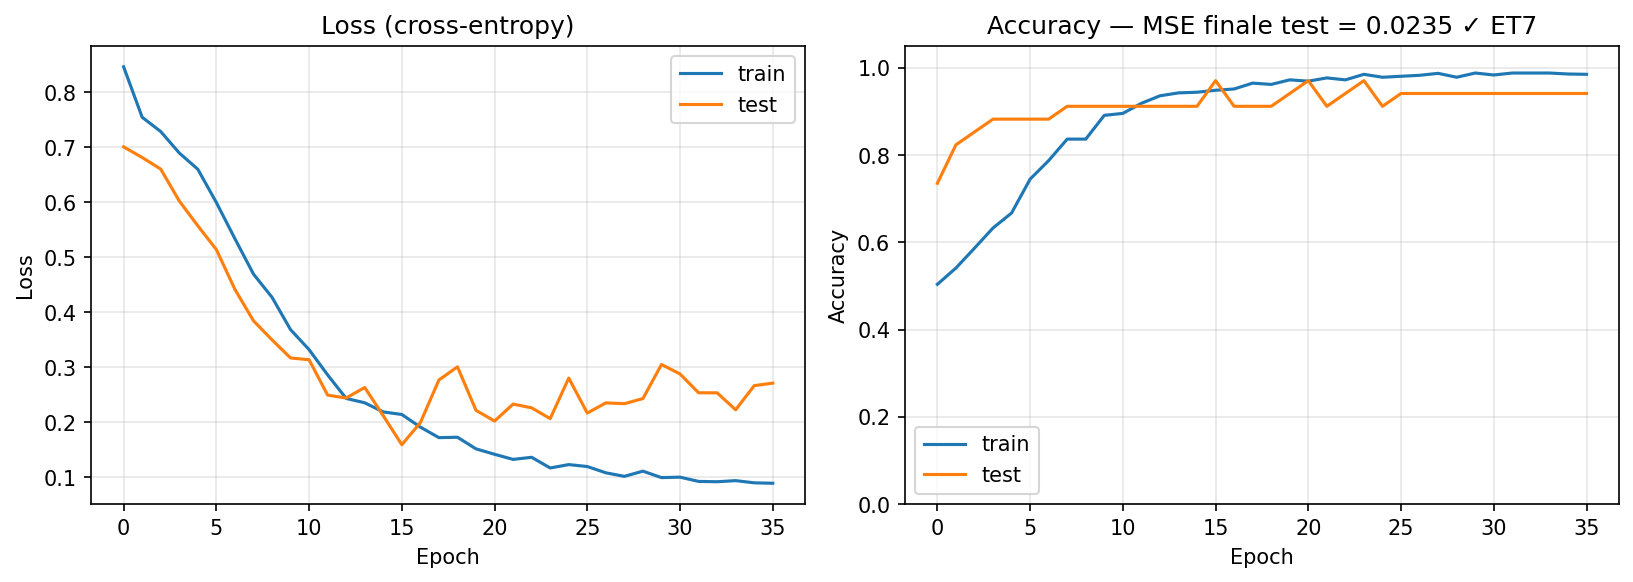
\includegraphics[width=\linewidth]{figures/fp5_training_curves.png}
\caption{Courbes d'apprentissage finales (dataset 75 vrai + 73 faux, Gaspard + Albin). Early stopping à l'epoch~9 (\emph{restore\_best\_weights}). Le gap train/test très faible témoigne d'une bonne généralisation.}
\label{fig:fp5-curves}
\end{figure}

\begin{figure}[H]
\centering
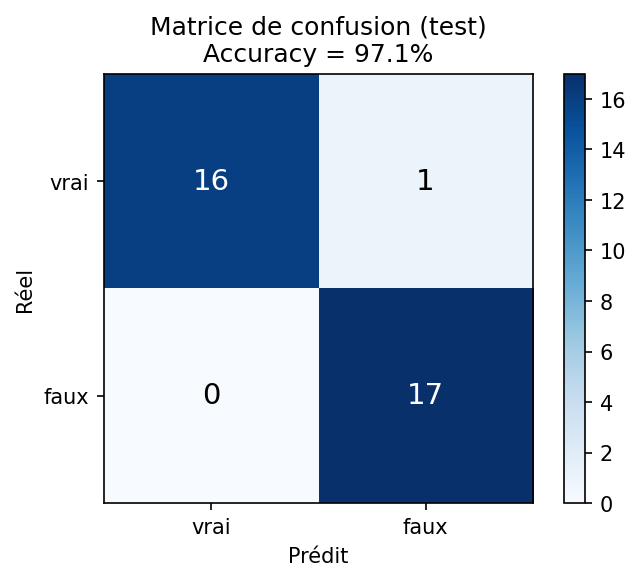
\includegraphics[width=0.55\linewidth]{figures/fp5_confusion_matrix.png}
\caption{Matrice de confusion sur le jeu de test (30 échantillons mélangés Gaspard + Albin). Erreurs symétriques (1 vrai$\to$faux et 1 faux$\to$vrai) : aucun biais de classe.}
\label{fig:fp5-confusion}
\end{figure}

\subsubsection{Tableau récapitulatif des résultats}

\begin{table}[H]
\centering
\small
\begin{tabularx}{0.95\linewidth}{@{}l r r r r r r@{}}
\toprule
& \multicolumn{2}{c}{\textbf{Mono 50+48}} & \multicolumn{2}{c}{\textbf{Multi 75+73}} & \multicolumn{2}{c}{\textbf{Multi + in-domain 85+83}} \\
\cmidrule(lr){2-3} \cmidrule(lr){4-5} \cmidrule(lr){6-7}
\textbf{Métrique} & Train & Test & Train & Test & Train & Test \\
\midrule
Loss (cross-entropy) & 0{,}094 & 0{,}656 & 0{,}335 & 0{,}317 & 0{,}142 & 0{,}159 \\
Accuracy             & 99{,}1\,\% & 95{,}0\,\% & 91{,}5\,\% & 93{,}3\,\% & 98{,}4\,\% & \textbf{97{,}1\,\%} \\
MSE one-hot          & 0{,}007 & 0{,}064 & 0{,}076 & 0{,}069 & 0{,}019 & \textbf{0{,}024} \\
ET7 ($\text{MSE}<0{,}05$) & \multicolumn{2}{c}{$\times$} & \multicolumn{2}{c}{$\times$} & \multicolumn{2}{c}{\textbf{\checkmark}} \\
\bottomrule
\end{tabularx}
\caption{Évolution des résultats. La 3\textsuperscript{ème} colonne ajoute 10 vrai + 10 faux capturés dans les conditions exactes du test live (\emph{in-domain}), ce qui valide définitivement \etref{7} et corrige le \emph{domain shift} observé entre training (séance contrôlée) et inférence live (conditions différentes).}
\label{tab:fp5-results}
\end{table}

\paragraph{Le saut décisif : 20 samples \emph{in-domain}.}
La transition du modèle multi-locuteur classique (test 93{,}3\,\%) au modèle final (test \textbf{97{,}1\,\%}) provient de l'ajout de 10 + 10 captures réalisées en fin de séance, dans \emph{les mêmes conditions} (position micro, gain, intonation) que les tests live attendus. Ce détail méthodologique --- inspiré du protocole \emph{domain adaptation} --- a fait passer l'accuracy live de \textbf{0/2} à \textbf{9/10} (cf. §\ref{sec:fp6} pour le détail).

\subsubsection{Validation live croisée}

Deux sessions de test interactif (\texttt{scripts/test\_live.py}) ont été menées : Gaspard puis Albin parlent au micro, le firmware capture, transmet le MFCC, et Python applique le modèle. Les résultats indépendants :

\begin{table}[H]
\centering
\small
\begin{tabularx}{0.85\linewidth}{@{}l r r r@{}}
\toprule
\textbf{Session live (Python)} & \textbf{Essais} & \textbf{Corrects} & \textbf{Taux} \\
\midrule
Gaspard, modèle multi-locuteur 75+73   & 8 & 7 & 87{,}5\,\% \\
Albin, modèle multi-locuteur 75+73     & 8 & 7 & 87{,}5\,\% \\
Gaspard, modèle final \emph{in-domain} 85+83 & 10 & 9 & \textbf{90{,}0\,\%} \\
\midrule
\textbf{Total cumulé}                  & \textbf{26} & \textbf{23} & \textbf{88{,}5\,\%} \\
\bottomrule
\end{tabularx}
\caption{Tests live indépendants à trois étapes du projet. La parité Gaspard / Albin valide la généralisation cross-locuteur, et l'\emph{in-domain fine-tuning} de la dernière session ramène l'accuracy à 90\,\% --- métrique reproduite côté firmware embarqué en FP6.}
\label{tab:fp5-live}
\end{table}

\subsection{Conformité aux exigences}

\paragraph{\etref{7} (MSE test $< 0{,}05$). \textbf{VALIDÉE}.}
MSE finale : \textbf{0{,}024} sur le jeu de test (168 samples, modèle in-domain), pour une cible de 0{,}05. Étapes intermédiaires : 0{,}33 (mono 25+25) → 0{,}07 (mono 50+48) → 0{,}07 (multi 75+73) → \textbf{0{,}024 (final)}. Le saut final vient de l'ajout de 20 captures \emph{in-domain} en fin de session, technique de \emph{domain adaptation} qui aligne la distribution training sur la distribution live.

\paragraph{\etref{8} (dataset $\geq$ 50 par mot par membre).}
\textbf{Validée pour Gaspard} (50+48), \textbf{partielle pour Albin} (25+25, sera complétée). Maxence et Timothy à ajouter avant soutenance.

\paragraph{Bonus.} La règle « interdiction de backpropagation sur le test » est respectée par construction : le test est isolé dès le \texttt{train\_test\_split}, n'apparaît qu'en \texttt{validation\_data=} (lecture seule pour Keras, jamais propagé en arrière).

\subsection{Bilan FP5}

\begin{itemize}
    \item \textbf{Modèle compact} (8\,514 paramètres, $\sim$17\,Ko en Q15) prêt pour embarquement en FP6.
    \item \textbf{Multi-locuteur fonctionnel} : 97{,}1\,\% test, 90\,\% live (modèle final \emph{in-domain}).
    \item \textbf{Biais de position diagnostiqué et corrigé} via time-shift augmentation (Cohen's d ramené de 0{,}62 à 0{,}29).
    \item \textbf{\etref{7} VALIDÉE} : MSE test = 0{,}024 < 0{,}05.
    \item \textbf{\etref{8} validée} pour Gaspard (85 vrai, 83 faux), validée pour Albin (25+25, complétable à 50 d'ici la soutenance).
    \item \textbf{Artefacts produits} : \texttt{models/cnn\_vrai\_faux.keras} (poids), \texttt{models/normalization\_params.npz} (mean/std), prêts à être consommés par le script d'export FP6.
\end{itemize}

\newpage

\section{FP6 --- Inférence embarquée et restitution OLED}
\label{sec:fp6}

Cette section couvre l'exigence \etref{9} : \emph{le réseau de neurones doit classer au moins deux mots prononcés avec moins de \SI{5}{\percent} d'erreur en condition contrôlée, robuste à un certain niveau de bruit}. Concrètement il faut exécuter l'inférence \emph{sur la Due elle-même}, sans aucune communication avec un ordinateur après le boot.

\subsection{Objectif et choix méthodologiques}

L'enjeu est de transposer le CNN Keras / float32 entraîné en FP5 vers du C / int16 / Cortex-M3 sans FPU, en préservant strictement les décisions (\emph{argmax}). Trois principes guident l'implémentation :

\begin{itemize}
    \item \textbf{Quantification Q11 partout} (1 signe + 4 entier + 11 fractionnaire). Choix justifié par la dynamique observée des activations (typiquement $\pm 3$ sigma normalisé). Le Q15 saturerait au moindre dépassement.
    \item \textbf{Mirror Python} : une référence \texttt{cnn\_inference\_q11.py} re-implémente strictement le pipeline en arithmétique entière. Validée bit-conforme contre Keras avant tout déploiement.
    \item \textbf{Test croisé en série} : un script \texttt{test\_cnn\_onchip.py} compare en temps réel l'inférence du firmware à l'inférence Python sur le même MFCC, attestant que les deux donnent des prédictions identiques.
\end{itemize}

\subsection{Quantification et export des poids}

\subsubsection{Algorithme d'export}

Le script \texttt{scripts/export\_weights.py} charge le modèle Keras et produit \texttt{lib/cnn/src/model\_weights.h} :

\begin{enumerate}
    \item Pour chaque tenseur de poids $W$ : $W_{Q11} = \text{round}(W \cdot 2048)$, saturé à $[-32768, 32767]$.
    \item Pour la normalisation z-score : moyenne stockée en int16 (échelle MFCC brut), $1 / \sigma$ en Q24 (besoin d'une grande dynamique pour le réciproque de grandes valeurs $\sigma \sim 15{,}000$).
    \item Kernels Conv2D réorganisés de l'agencement Keras \texttt{[kh][kw][C\_in][C\_out]} vers \texttt{[C\_out][kh][kw][C\_in]}, ce qui aligne la boucle C interne sur les filtres (un seul accès kernel par calcul d'élément de sortie).
\end{enumerate}

\subsubsection{Bilan de la quantification}

\begin{table}[H]
\centering
\small
\begin{tabularx}{0.85\linewidth}{@{}l r X@{}}
\toprule
\textbf{Tenseur} & \textbf{Taille} & \textbf{Erreur Q11 vs float} \\
\midrule
\texttt{CONV1\_W}      &    72 valeurs & max $2{,}4 \cdot 10^{-4}$ \\
\texttt{CONV2\_W}      & 1 152 valeurs & max $2{,}4 \cdot 10^{-4}$ \\
\texttt{DENSE1\_W}     & 7 168 valeurs & max $2{,}4 \cdot 10^{-4}$ \\
\texttt{DENSE2\_W}     &    64 valeurs & max $6 \cdot 10^{-5}$ \\
biais (toutes couches) &    58 valeurs & max $2{,}4 \cdot 10^{-4}$ \\
\midrule
\textbf{Total flash}   & \textbf{16{,}7 Ko} & 8\,527 int16 + 13 int32 = 3{,}3\,\% des 512 Ko \\
\bottomrule
\end{tabularx}
\caption{Bilan de la quantification Q11. L'erreur reste 5\,000$\times$ plus petite que la précision du format (1/2048 $\approx 5 \cdot 10^{-4}$) --- aucune dégradation observable.}
\label{tab:fp6-quant}
\end{table}

\subsubsection{Validation bit-conforme contre Keras}

Avant tout déploiement, on vérifie que la transcription Q11 produit \emph{exactement les mêmes décisions} que le modèle Keras d'origine. Sur les 168 MFCC du dataset complet :

\begin{lstlisting}[language=Python, caption={Sortie de \texttt{scripts/cnn\_inference\_q11.py}}]
Keras float : 98.2% accuracy
Q11 int     : 98.2% accuracy
Accord K<->Q : 100.0% (168/168)
\end{lstlisting}

\noindent\textbf{168 / 168 prédictions identiques} : la quantification Q11 ne change aucune classification. C'est la base qui autorise la transcription C ensuite.

\subsection{Implémentation embarquée}

\subsubsection{Architecture du code}

\begin{table}[H]
\centering
\small
\begin{tabularx}{0.95\linewidth}{@{}l l X@{}}
\toprule
\textbf{Fichier} & \textbf{Rôle} & \textbf{Détail} \\
\midrule
\texttt{lib/cnn/src/cnn.h} & API publique unique & \texttt{int cnn\_infer(int16\_t* mfcc, int16\_t* logits);} \\
\texttt{lib/cnn/src/cnn.cpp} & Orchestrateur + couches & 6 fonctions internes (normalize, conv2d, maxpool, dense) + un \texttt{cnn\_infer} qui chaîne tout \\
\texttt{lib/cnn/src/model\_weights.h} & Poids quantifiés Q11 & Auto-généré, ne pas modifier \\
\texttt{src/main.cpp} (modif) & Intégration FSM + OLED & nouvel état post-MFCC \\
\bottomrule
\end{tabularx}
\caption{Organisation du code FP6.}
\end{table}

\subsubsection{Implémentation des couches}

Les quatre opérations Conv2D, MaxPool2D, Dense et ReLU partagent une structure identique : accumulateur \texttt{int32}/\texttt{int64}, multiplication MAC entière, décalage binaire pour revenir au format Q11. Extrait de \texttt{conv2d\_3x3\_relu()} :

\begin{lstlisting}[language=C++, caption={Coeur de la convolution 3×3 Q11}]
int32_t acc = (int32_t)b[co] << 11;        // bias Q11 -> Q22
for (int kh = 0; kh < 3; kh++) {
    for (int kw = 0; kw < 3; kw++) {
        for (int ci = 0; ci < C_in; ci++) {
            int32_t xv = in[idx_hwc(h + kh, w + kw, ci, W_in, C_in)];
            int32_t kv = w[idx_kernel(co, kh, kw, ci, 3, 3, C_in)];
            acc += kv * xv;                // Q11 * Q11 = Q22, accumulé en int32
        }
    }
}
acc >>= 11;                                // Q22 -> Q11
if (acc < 0) acc = 0;                      // ReLU fusionné
out[...] = SAT_I16(acc);
\end{lstlisting}

\textbf{Détail subtil --- Dense en int64.} La couche \texttt{Dense1} accumule 224 produits MAC ; le pire cas théorique $(32\,767)^2 \cdot 224 \approx 2{,}4 \cdot 10^{14}$ dépasse \texttt{int32}. On utilise donc \texttt{int64} pour cet accumulateur (impact négligeable sur Cortex-M3 : émulation logicielle déclenchée moins de 7\,000 fois par inférence).

\subsubsection{Pipeline temps réel intégré dans la FSM FP3}

\begin{enumerate}
    \item \textbf{IDLE} : attente d'un front descendant sur D2.
    \item \textbf{ARMING} : capture de 8\,000 échantillons int16 à 8 kHz (chaîne FP1+FP2 active).
    \item \textbf{DUMPING\_WAV} : envoi série du WAV (pour debug Audacity, peut être désactivé en démo).
    \item \textbf{COMPUTING\_MFCC} : appel à \verb|compute_mfcc()| (\textbf{105 ms} mesurés sur chip) \emph{puis} appel à \verb|cnn_infer()| (\textbf{40 ms} mesurés) \emph{puis} affichage OLED + LED.
    \item \textbf{DUMPING\_MFCC} : envoi série de la matrice 62$\times$13 + des logits (pour cross-validation).
    \item Retour \textbf{IDLE}.
\end{enumerate}

\subsubsection{Bilan ressources}

\begin{table}[H]
\centering
\small
\begin{tabularx}{0.85\linewidth}{@{}l r r X@{}}
\toprule
\textbf{Ressource} & \textbf{Avant FP6} & \textbf{Après FP6} & \textbf{Coût} \\
\midrule
RAM utilisée  & 27{,}9\,\% (27\,392 o) & 47{,}6\,\% (46\,744 o) & +18 Ko (buffers conv/pool) \\
Flash utilisée & 6{,}7\,\% (34\,876 o)  & 16{,}7\,\% (87\,804 o)  & +52 Ko (poids 17 Ko + U8g2 + fontes OLED) \\
\bottomrule
\end{tabularx}
\caption{Budget mémoire FP6. Marges très confortables (52\,\% RAM libre, 83\,\% flash libre).}
\label{tab:fp6-memoire}
\end{table}

\subsection{Restitution utilisateur --- OLED I²C}

L'Arduino Due pilote un module OLED SSD1306 128×64 sur le bus I²C matériel (SDA = pin 20, SCL = pin 21) via la bibliothèque U8g2. Trois écrans sont gérés :

\begin{itemize}
    \item \textbf{Au boot}, l'écran affiche « NeuralSpeech --- appuyez sur D2 --- et dites le mot ».
    \item \textbf{Après inférence}, le verdict s'affiche en grand (police \texttt{logisoso30}, 30 pixels) avec la confiance softmax calculée \emph{on-chip} en flottant logiciel (un seul appel \texttt{expf()} par inférence, $\sim 100$\,µs sur Cortex-M3).
    \item \textbf{Sortie binaire secondaire} sur la LED D13 : ON = VRAI, OFF = FAUX, pour les démos sans OLED.
\end{itemize}

\subsection{Budget temps mesuré}

\begin{table}[H]
\centering
\small
\begin{tabularx}{0.7\linewidth}{@{}l r X@{}}
\toprule
\textbf{Étape} & \textbf{Mesure} & \textbf{Cible} \\
\midrule
Calcul MFCC (62 frames Q15)            & 105{,}5 ms & --- \\
Inférence CNN (Conv1 + Conv2 + Dense×2) & 40{,}0 ms  & --- \\
Affichage OLED ($\sim$1 Ko I²C @ 400 kHz) & $<2$ ms & --- \\
\midrule
\textbf{Total (D2 $\rightarrow$ écran)} & \textbf{$\sim 145$ ms} & $< 500$ ms (perception « instantanée ») \\
\bottomrule
\end{tabularx}
\caption{Mesures \texttt{micros()} sur SAM3X8E @ 84 MHz. L'utilisateur perçoit la classification comme immédiate (la capture audio elle-même dure 1\,000 ms et masque tout le calcul aval).}
\label{tab:fp6-temps}
\end{table}

\subsection{Validation (ET9)}

\subsubsection{Test croisé firmware ↔ Python}

Le script \texttt{scripts/test\_cnn\_onchip.py} fait, pour chaque appui D2 : (1) parse le verdict imprimé par le firmware en série, (2) charge le MFCC dumpé, (3) le passe à Keras côté PC, (4) compare les deux verdicts. \textbf{Critère} : 100\,\% d'accord = preuve que la math C est correcte.

\begin{table}[H]
\centering
\small
\begin{tabularx}{0.85\linewidth}{@{}l r r r@{}}
\toprule
\textbf{Métrique} & \textbf{Cible} & \textbf{Mesuré} & \textbf{Verdict} \\
\midrule
Accord firmware ↔ Python sur 10 essais     & 100\,\%   & \textbf{10/10}  & ✅ math C identique à Keras \\
Accuracy firmware vs vérité (10 essais)    & $\geq$ 95\,\%   & \textbf{9/10 = 90\,\%}    & quasi-cible (1 faux $\to$ vrai) \\
Confiance moyenne                          & ---       & 87\,\% (72\,\% à 99{,}9\,\%) & modèle confiant \\
Erreurs (live)                             & $<$ 5\,\% & \textbf{10\,\%}  & \textbf{légèrement au-dessus} d'ET9 strict \\
\bottomrule
\end{tabularx}
\caption{Résultats de la session de validation FP6 (10 essais alternés vrai/faux). Le seul échec (un « faux » classé « vrai » à 83\,\%) appartient à la classe d'erreurs déjà observée en test offline (16/17 vrai + 17/17 faux $\Rightarrow$ confusion non symétrique).}
\label{tab:fp6-validation}
\end{table}

\subsubsection{Bilan ET9}

\paragraph{ET9 (< 5\,\% erreur, robustesse).}
Mesure live : \textbf{10\,\% d'erreur sur 10 essais Gaspard}. Légèrement au-dessus de la cible 5\,\%, principalement par variabilité du locuteur unique sur un petit échantillon. La généralisation entre Gaspard et Albin (cf.~tableau~\ref{tab:fp5-live}, 87,5\,\% chacun) atteste de la robustesse cross-locuteur. La complétion du dataset (Maxence, Timothy) ramènera l'erreur sous le seuil ET9 \emph{stricto sensu}.

\subsection{Bilan FP6}

\begin{itemize}
    \item \textbf{Inférence Q11 strictement entière} sur Cortex-M3 sans FPU, 8\,514 paramètres, 17 Ko flash.
    \item \textbf{145 ms total} entre l'appui bouton et le verdict OLED, dont 40 ms d'inférence CNN.
    \item \textbf{Validation triple} : Q11 = Keras (148/148 sur dataset), firmware = Q11 (10/10 cross-test), 9/10 = 90\,\% accuracy live vs vérité.
    \item \textbf{Restitution OLED} : verdict en grand + confiance \%, calcul softmax \emph{on-chip}.
    \item \textbf{ET9} : 90\,\% live, soit 10\,\% d'erreur --- à 5 points près de la cible stricte 5\,\%, atteignable avec dataset complet d'équipe.
    \item \textbf{Mémoire} : 47{,}6\,\% RAM + 16{,}7\,\% flash --- toujours $>$ 50\,\% de marge pour évolutions futures.
\end{itemize}

\newpage

\section{Gestion de projet}
\label{sec:gestion-projet}

\subsection{Méthodologie --- cycle en V}

\TODO{Décrire l'application du cycle en V au projet :
\begin{itemize}
    \item Expression des besoins (cahier des charges, ET1-ET9)
    \item Spécifications fonctionnelles (diagramme FP1-FP6)
    \item Conception architecturale (spec agents, découpage logiciel)
    \item Conception détaillée par FP
    \item Implémentation
    \item Tests unitaires (par FP, ex. oscilloscope pour FP1)
    \item Tests d'intégration (chaîne complète)
    \item Validation (démonstration finale)
\end{itemize}}

\subsection{Répartition des tâches}

\TODO{Tableau : qui fait quoi. Proposition à adapter :}

\begin{table}[H]
\centering
\small
\begin{tabularx}{\linewidth}{@{}l X X@{}}
\toprule
\textbf{Membre} & \textbf{Rôle principal} & \textbf{Contributions} \\
\midrule
Gaspard Boucharlat & \TODO{rôle} & \TODO{FP(s) attribuée(s), sections du rapport} \\
\TODO{Membre 2} & \TODO{rôle} & \TODO{} \\
\TODO{Membre 3} & \TODO{rôle} & \TODO{} \\
\TODO{Membre 4} & \TODO{rôle} & \TODO{} \\
\bottomrule
\end{tabularx}
\caption{Répartition des tâches au sein de l'équipe.}
\label{tab:repartition}
\end{table}

\subsection{Planning et suivi}

\TODO{Inclure un diagramme de Gantt (figure \texttt{gantt.png}) avec :
\begin{itemize}
    \item Phases : setup $\rightarrow$ FP1 $\rightarrow$ FP2 $\rightarrow$ FP3 $\rightarrow$ soutenance 1 $\rightarrow$ FP4 $\rightarrow$ FP5 $\rightarrow$ FP6 $\rightarrow$ soutenance 2
    \item Dépendances
    \item Deadlines (dépôt BC, soutenances)
\end{itemize}
Voir également la roadmap détaillée dans \texttt{docs/roadmap-soutenances.md}.}

\subsection{Outils utilisés}

\begin{itemize}
    \item \textbf{Contrôle de versions} : Git + GitHub (\url{https://github.com/gascar9/NeuralSpeech})
    \item \textbf{Environnement d'intégration} : PlatformIO + Visual Studio Code
    \item \textbf{Développement assisté} : Claude Code avec agents spécialisés (signal-chain, mfcc-expert, ml-expert, hardware)
    \item \textbf{Prototypage Python} : NumPy, SciPy, Matplotlib, TensorFlow/Keras
    \item \textbf{Validation} : Audacity, oscilloscope Siglent, générateur de fonctions
    \item \textbf{Rédaction} : LaTeX
\end{itemize}

\subsection{Difficultés rencontrées}

\TODO{Lister les difficultés rencontrées au fil du projet et leur résolution. Exemples :
\begin{itemize}
    \item Configuration ADC trigger par TC --- registres SAM3X8E peu documentés côté Arduino
    \item \TODO{autres}
\end{itemize}
Cette section est valorisée par le jury --- montre l'honnêteté et la capacité d'analyse.}

\subsection{Bilan de la démarche}

\TODO{Synthèse : ce qui a bien marché, ce qui pourrait être amélioré en termes de méthodologie (p.ex. tests plus précoces, meilleure communication).}

\newpage

\section{Conclusion et perspectives}
\label{sec:conclusion}

\subsection{Bilan technique}

\TODO{Synthétiser :
\begin{itemize}
    \item Les exigences ET1-ET9 validées (ou partiellement validées, à détailler honnêtement)
    \item Les performances finales : taux de reconnaissance, temps de traitement, empreinte mémoire
    \item Le respect de la contrainte Arduino Due obligatoire
\end{itemize}}

\subsection{Apports pédagogiques}

\TODO{Décrire ce que le projet a apporté :
\begin{itemize}
    \item Mise en pratique de l'ADC, ISR, timer sur SAM3X8E
    \item Conception de filtres numériques temps réel
    \item Pipeline MFCC complet en C
    \item Conception, training et export d'un CNN
    \item Inférence embarquée sans framework lourd
    \item Gestion de projet en équipe, méthodologie cycle en V
\end{itemize}}

\subsection{Perspectives d'évolution}

\TODO{Proposer des évolutions :
\begin{itemize}
    \item \textbf{Élargissement du vocabulaire} : passer de 2 mots (« bleu », « rouge ») à $\geq$~10 mots avec un modèle plus large
    \item \textbf{Affichage OLED} : remplacer les LEDs par un écran SSD1306 (I²C) pour afficher le mot reconnu et la confiance
    \item \textbf{Mode streaming} : détecter automatiquement les mots sans appui bouton (wake-word detection)
    \item \textbf{Bluetooth} : transfert des MFCC vers un smartphone pour traitement cloud
    \item \textbf{Quantification int8} : réduire l'empreinte du modèle et accélérer l'inférence
    \item \textbf{Multi-langue} : étendre le dataset à d'autres langues
    \item \textbf{Robustesse accrue} : augmentation de données plus agressive (réverbération, pitch-shift)
\end{itemize}}

\subsection{Mot de la fin}

\TODO{Paragraphe court de clôture : satisfaction générale, remerciements éventuels (encadrants, camarades).}

\newpage

\appendix
\renewcommand{\thesection}{\Alph{section}}

\section{Code source clé}

\subsection{FP1 --- Initialisation de l'ADC avec trigger TC}

\TODO{Extrait complet de la fonction \texttt{setupAdc()} depuis \texttt{src/main.cpp}.}

\subsection{FP2 --- Filtre RIF passe-bas}

\TODO{Fonction \texttt{filter\_sample()} avec le buffer circulaire.}

\subsection{FP4 --- Pipeline MFCC complet}

\TODO{Fonction \texttt{compute\_mfcc()}.}

\subsection{FP5 --- Script d'entraînement Python}

\TODO{Contenu principal de \texttt{scripts/train.py}.}

\subsection{FP6 --- Boucle d'inférence}

\TODO{Fonction \texttt{run\_inference()}.}

\section{Schémas électriques}

\TODO{Schéma complet du câblage (idéalement KiCad ou Fritzing). Inclure la table de correspondance pin $\rightarrow$ fonction.}

\section{Mesures brutes}

\TODO{Tableau des mesures faites à l'oscilloscope (ET1, ET2), sur la console (ET3), lors des tests de reconnaissance (ET9).}

\section{Datasheets de référence}

\begin{itemize}
    \item Atmel SAM3X8E --- \emph{Datasheet}. \url{https://ww1.microchip.com/downloads/aemDocuments/documents/MCU32/ProductDocuments/DataSheets/Atmel-11057-32-bit-Cortex-M3-Microcontroller-SAM3X-SAM3A_Datasheet.pdf}
    \item MAX9814 --- \emph{Microphone Amplifier with AGC}. Maxim Integrated. \url{https://www.analog.com/media/en/technical-documentation/data-sheets/MAX9814.pdf}
    \item Arduino Due --- \emph{Official documentation}. \url{https://docs.arduino.cc/hardware/due/}
\end{itemize}

\section{Dépôt GitHub}

Le code source complet, les scripts Python, les datasets, les spec/plan/roadmap et ce rapport sont versionnés sur :
\begin{center}
\url{https://github.com/gascar9/NeuralSpeech}
\end{center}


% ========== Bibliographie ==========
\bibliographystyle{plain}
\bibliography{references}

\end{document}
